\chapter{Theoretical background}\label{ch:2}

The main objectives of this chapter are to define the key concepts of L2 speech acquisition, to give insight into a study of intonation, to compare sound systems of the languages under study and to discuss relevant theories and models in the light of an exhaustive review of the literature that is relevant to the present study. The first section (\sectref{sec:2.1}) deals with several important factors affecting L2 speech (L1 background, L2 proficiency level, age of learning, role of input, phonological awareness, personal variables and other influences) and presents a large discussion on this matter (\sectref{sec:2.1.1}--\sectref{sec:2.1.7}). The second section (\sectref{sec:2.2}) is devoted to the definition and modelling of the suprasegmental phenomenon -- intonation. It provides a detailed description of the Autosegmental-Metrical Model (AM model) (\sectref{sec:2.2.1}) and the Tones and Break Indices (ToBI) annotation system (\sectref{sec:2.2.2}), which are both crucial for the current study. In addition, I will offer a set of AM-based labels chosen for the analysis of the present L2 data (\sectref{sec:2.2.3}). The third section (\sectref{sec:2.3}) outlines and compares phonological systems of the languages under study, taking into account segmental (\sectref{sec:2.3.1}) as well as suprasegmental features and the prosodic typology of languages (\sectref{sec:2.3.2}). The last section of the chapter (\sectref{sec:2.4}) introduces and discusses several important models and techniques of L2 speech acquisition, placing a special focus on \citegen{Mennen2015} L2 Intonation Learning theory.

\section{Factors affecting L2 speech}\label{sec:2.1}

Since it is true that language is inherently variable, it is also true that L2 languages are full of target-like variation patterns \citep[272]{Regan2013}.  Interlanguage production (and perception) is very characteristic of inter-learner variability (differences between learners) and intra-learner variability (variability within the same learner). The present study will concentrate on two main learner-related sources of variability taken into account for explaining variation patterns in an L2: the \textit{L1 background} (Czech vs. German) and \textit{L2 proficiency} (intermediate level vs. advanced level). My starting point is a very general assumption that the first language plays a key role in L2 speech (see, e.g., \citealt{Suter1976}). For example, it is not difficult for a native speaker to distinguish among Czech, Italian, Spanish and German accents in English.\footnote{There are two interesting online archives for listening to different accents in (L2) English: the \textit{International Dialects of English Archive} \citep{Meier1998} and the \textit{Speech Accent Archive} \citep{Weinberger2015}. Equivalent resources for L2 Spanish and L2 Italian do not exist, although some first steps have been made in this regard for Spanish (see, for example, the IFEC corpus project -- \textit{(Inter-)Fonología del Español Contemporáneo} -- presented in \chapref{ch:3}).} The first factor (\sectref{sec:2.1.1}) should elucidate production errors and interferences and explain the role of L1 in L2 speech in general. The second factor (\sectref{sec:2.1.2}) should explain whether errors attributable to \textit{transfer} decrease in more advanced learners and how the developmental sequences (may) change over time. It is suggested that with regard to language level, Czech and German learners of an advanced level should become more similar in their L2 Spanish than those of an intermediate level. In a similar way, it is to be expected that intermediate L2 Italian learners (L1 Czech) will resemble intermediate L2 Spanish learners (L1 Czech) and that the advanced groups will present more different intonational patterns. In the following sections, some other traditional factors asserted to affect L2 speech such as age of acquisition, the role of input, phonological awareness, gender and personal factors will also be reviewed (\sectref{sec:2.1.3}--\sectref{sec:2.1.7}). As we will see, there are several disagreements and even contradictory conclusions regarding the effect of different factors, which makes understanding of the interlanguage somewhat puzzling (for overviews and discussion see, e.g., \citealt{PiskeEtAl2001, ColantoniEtAl2015, DerwingMunro2015}). For example, whereas \citet[201]{PiskeEtAl2001} report “little evidence that amount of formal instruction as such affects degree of L2 foreign accent”, the majority of the studies reviewed by \citet{DerwingMunro2015} show that formal instruction such as specific training techniques yielded positive results in L2 accuracy. The reasons for the (partly) conflicting findings may be the study of different languages, examination of different phenomena, application of different experimental methods and measurements, or the complex nature of the L2 speech. In spite of several opposite and ambiguous results, it is, however, of utmost importance to control for different variables (see \citealt[5]{ColantoniEtAl2015}) because they can be very useful for the latter interpretation of the data and for gaining a deeper insight into the phenomenon under study.

\subsection{L1 background}\label{sec:2.1.1}\largerpage[2]

As already presented in the \textit{Introduction}, L2 speech is characterized by a phenomenon denoted as cross-linguistic influence (CLI), language transfer or interference, which has an impact on all aspects of segmental and suprasegmental phonology. CLI or language transfer refers to the fact that L2 learners use L1 categories in their L2 production as well as their L2 perception (e.g., \citealt{Gass1984,Gass1996, Odlin1989,Odlin2003, Selinker1993, ColantoniEtAl2015}). One of the main reasons for this is that L2 learners mostly concentrate on meaning rather than form and because they are not starting from true “zero” in linguistic terms and therefore require “the overriding of the pre-existing L1 neural connections” (\citealt[90]{Kivistö-deSouza2015}; see \citealt{N.C.Ellis2002} and \citealt{R.Ellis2009} for a discussion on the relationship between the SLA theory and the neuroscience of learning and memory). It is thus reasonable to assume that the L1 background is the main determinant of L2 speech.


It is important to keep in mind that \textit{accentedness} in L2 (the extent to which a listener judges L2 speech according to the native speaker norm, see, e.g., \citealt{Piske2008}) is not the same as \textit{identification} of the speaker (recognition of where the L2 speaker is from, see, e.g., \citealt{KollyDellwo2013}). We can generally make a good guess about where the speaker comes from. So, for example, one Czech and one German speaker may be both evaluated to have a very weak foreign accent, but we may be able to hear differences between them and very possibly say who is German and who is Czech. If the influence of L1 is expected, the following questions may arise: \textit{Do German learners of Spanish differ substantially from Czech learners of Spanish in terms of intonation? Are there any tonal features typical of German or Czech learners in particular? If so, do we find the same features in two different target languages (Italian and Spanish) produced by learners coming from the same L1 background?} These and other questions will accompany this study. In the following sections, I will discuss some traditional factors claimed to affect L2 speech. Specific hypotheses of the present study based on cross-linguistic influence will be formulated in \chapref{ch:4}.


\subsection{L2 proficiency level}\label{sec:2.1.2}\largerpage[2]

Second language proficiency or the ability of an individual to speak and perform in an L2 is another factor expected to explain the variability observed in L2. For example, the study by \citet{CroccoBaele2012} on yes/no questions in L2 Italian by L1 Dutch speakers has shown that advanced learners produce more native-like patterns compared with less experienced learners. In a similar way, a longitudinal study by \citet{MennenEtAl2010} has shown that Italian and Punjabi learners of English make certain improvements in L2 intonation (e.g., the use of certain target-like patterns) over the course of their stay in the host country.


Due to the fact that the present research is not longitudinal in nature, its main idea is to compare intermediate (B level) and advanced (C level) learners in order to find out whether there are any differences between the two groups and whether there is positive movement towards a native-like production in terms of intonation. Such a cross-sectional approach has been to date the most common way to account for L2 development.



The proficiency level of the learners examined in the present study was determined according to the CEFR guideline (\citealt{CEFR2001,CEFR2011, CEFR2018}), which describes the achievements of learners of L2 languages and is commonly used across Europe, including Germany and the Czech Republic. All the participants of the present study self-reported their foreign language proficiency levels in accordance with the courses they were attending (or had recently finished) at the time of the experiment. No specific tests for measurements of participants’ phonological or other linguistic competences were carried out, but the learners were asked to answer a set of predetermined questions in a semi-directed interview (see \sectref{sec:3.2} for details), the aim of which was to detect, among other things, their explicit L2 phonological awareness (see \sectref{sec:2.1.6}). It should be pointed out that the determination of participants’ levels within the “traditional” proficiency frameworks (and the present study too) is actually based on grammar, vocabulary, oral and written expression and overall communication skills rather than on phonological competence. The target skills for spoken interaction and production as stipulated by the CEFR essentially focus on (speech) intelligibility, “the most fundamental characteristic of successful oral communication” (\citealt[1]{DerwingMunro2015}). \tabref{tab:2.1} offers a full description of spoken competences of learners at B and C levels as proposed in \citet{CEFR2018}.


\begin{table}
\begin{tabularx}{\textwidth}{lX}
      \lsptoprule
      \multicolumn{2}{l}{Independent (intermediate) users}\\\midrule
      B1 & I can connect phrases in a simple way in order to describe experiences and events, my dreams, hopes and ambitions. I can briefly give reasons and explanations for opinions and plans. I can narrate a story or relate the plot of a book or film and describe my reactions.\\
      B2 & I can present clear, detailed descriptions on a wide range of subjects related to my field of interest. I can explain a viewpoint on a topical issue giving the advantages and disadvantages of various options.\\\midrule
      \multicolumn{2}{l}{Proficient (advanced) users}\\\midrule
      C1 & I can present clear, detailed descriptions of complex subjects integrating sub-themes, developing particular points and rounding off with an appropriate conclusion.\\ 
      C2 & I can present a clear, smoothly flowing description or argument in a style appropriate to the context and with an effective logical structure which helps the recipient to notice and remember significant points.\\
      \lspbottomrule
  \end{tabularx}
\caption{Spoken skills for levels B and C according to the \citet{CEFR2018}.}
\label{tab:2.1}
\end{table}

In real life and many language courses, pronunciation still plays a relatively secondary role in an individual’s language proficiency. And as \citet[47]{CEFR2018} admits, “[p]honology had been the least successful scale developed in the research behind the original descriptors.” Nevertheless, this does not mean that phonology is completely ignored in the CEFR proposals. Let us here make a short digression to look at the latest proposals in this regard and start with the illustrative descriptor scale proposed already in 2001 for the assessment of foreign language proficiency (\tabref{tab:2.2}).

\begin{table}
	\begin{tabularx}{\textwidth}{lX}
		\lsptoprule
		\multicolumn{2}{l}{Independent (intermediate) users}\\\midrule
		{B1} & Pronunciation is clearly intelligible even if a foreign accent is sometimes evident and occasional mispronunciations occur.\\
	    {B2} & Has a clear, natural pronunciation and intonation.\\\midrule
	    \multicolumn{2}{l}{Proficient (advanced) users}\\\midrule
	    {C1} & Can vary intonation and place sentence stress correctly in order to express finer shades of meaning.\\
	    {C2} & {\itshape No descriptor available}\\
		\lspbottomrule
	\end{tabularx}
	\caption{Phonology scale according to the \citet{CEFR2001}.}
	\label{tab:2.2}
\end{table}

Although this proposed scale for phonological skills is transparent, comprehensive and broad enough to capture new directions in L2 learning and teaching, it has not gained widespread acceptance, for three main reasons. First, it is oriented (implicitly) around the native speaker norm. Second, its main focus is on intelligibility (“clearly intelligible”, “a clear pronunciation”, “finer shades of meaning”) and comprehensibility (“can be understood”) rather than on any concrete pronunciation skills (for example, intonation skills are mentioned first at the B2 level, even though this aspect is present in the target language from the very beginning of acquisition, in contrast to certain vocabulary or grammatical categories). And third, the treatment of foreign accent does not reflect reality. As we have noted, a foreign accent seems to be in effect “tolerated” until the B1 level; from this level on learners are presumed to have mastered L2 pronunciation “perfectly”. Notice that there is no descriptor available for C2 at all, which again implies that phonological skills must be fully acquired not later than the C1 level, which is quite an unrealistic ambition. This is also critical because a foreign accent is very negatively seen at this level and from research we know that even highly advanced C2 speakers still may have a foreign accent. In an update, the CEFR \textit{Phonology} sub-project (\citealt{Piccardo2016, CEFR2018}) conducted various validation phases in relation to other new scales described below, with over 250 informants involved in each phase, and based on their results proposed a new phonological skills rubric for \citealt{CEFR2018} (\tabref{tab:2.3a}). This recent proposal is more extensive and comprises besides the overall phonological control two other core areas: sound recognition and articulation and prosodic features (including intonation, stress and rhythm). I present only the first and the last area here.\largerpage

\begin{table}
	\caption{Overall phonological control according to \citealt{CEFR2018}.}
	\label{tab:2.3a}
	\begin{tabularx}{\textwidth}{lX}
		\lsptoprule
		\multicolumn{2}{l}{{Independent (intermediate) users}}\\\midrule
		{B1} & Pronunciation is generally intelligible; can approximate intonation and stress at both utterance and word levels. Accent is generally influenced by other language(s) he/she speaks, and this may occasionally affect intelligibility.\\
		{B2} & Can generally use appropriate intonation, place stress correctly and articulate individual sounds clearly.
		
		Accent tends to be influenced by other language(s) he\slash she speaks, but has little or no effect on intelligibility.\\\midrule
		\multicolumn{2}{l}{{Proficient (advanced) users}}\\\midrule
		{C1} & Can employ the full range of phonological features in the target language with sufficient control to ensure intelligibility throughout.
		
		Can articulate virtually all the sounds of the target language; some features of accent retained from other language(s) may be noticeable, but they do not affect intelligibility at all.\\
		{C2} & Can employ the full range of phonological features in the target language with a high level of control -- including prosodic features such as word and sentence stress, rhythm and intonation -- so that the finer points of his/her message are clear and precise.
		
		Intelligibility and effective conveyance and enhancement of meaning are not affected in any way by features of accent that may be retained from other language(s).\\
		\lspbottomrule
	\end{tabularx}
\end{table}

\begin{table}
	\caption{Phonology control (prosodic features) according to \citealt{CEFR2018}}
	\label{tab:2.3b}
	\begin{tabularx}{\textwidth}{lX}
		\lsptoprule
		\multicolumn{2}{l}{{Independent (intermediate) users}}\\\midrule
		B1 & Can convey his/her message in an intelligible way in spite of a strong influence on stress, intonation and/or rhythm from other language(s) he/she speaks.\\
		B2 & Can employ prosodic features (e.g. stress, intonation, rhythm) to support the message he/she intends to convey, though with some influence from other languages he/she speaks.\\\midrule
		\multicolumn{2}{l}{{Proficient (advanced) users}}\\\midrule
		C1 & Can produce smooth, intelligible spoken discourse with only occasional lapses in control of stress, rhythm and/or intonation, which do not affect intelligibility or effectiveness. Can vary intonation and place sentence stress correctly in order to express precisely what he/she means to say.\\
		C2 & Can exploit prosodic features (e.g. stress, rhythm and intonation) appropriately and effectively in order to convey finer shades of meaning (e.g. to differentiate and emphasise). \\
		\lspbottomrule
	\end{tabularx}
\end{table}

The main difference with regard to the earlier proposal is that foreign accent is not completely excluded at the higher levels and it is not negatively perceived as long as it does not impede clarity and intelligibility. Today, the majority of experts agree that the \textit{Intelligibility Principle} (in terms of \citealt{Levis2005}) is more appropriate than \textit{nativeness} as a basic orientation to pronunciation instruction (see, e.g., \citealt{Piccardo2016, DerwingMunro2015}). This does not mean, however, that pronunciation is of little importance. Regarding the phenomenon under study here, learners at the B levels should use \textit{appropriate} intonation in order to “support message correctly” and those at the C levels should be able to use intonation \textit{appropriately} and \textit{effectively} in order to “convey finer shades of meaning”. Although this latest proposal is important, in my opinion, it is still very general and lacks information on what intonation parameters should be acquired exactly. Based on the findings of the present study, I will later offer a preliminary scheme on intonation scale or skills that can be integrated into the \textit{Phonology control} within the CEFR (see \chapref{ch:5}, \sectref{sec:5.2.1}). On the other hand, the particular strength of the proposal is that phonological skills, which were based on observations of L2 speakers with different L1 backgrounds, cover various phonetic and phonological phenomena and are not exclusively oriented around the native norm. That said, however, it should not be forgotten that the CEFR proposal is strongly Anglocentric as it was developed according to the \textit{lingua franca} English. Hence, the prosodic typology and prosodic systems of the individual target languages as well as issues such as the distance between the L1 and the target language are not taken into account here. It also raises the question as to how to implement such phonological assessment in language courses, which would imply a need to develop materials for both learners and teachers, to say nothing of the possible revising of language policy documents and teacher education in general \citep{Piccardo2016}.


Finally, it should be pointed out that the observations made by the new CEFR phonological assessment tool show that there are differences between the two levels (B and C) in terms of prosody; and, hence, a comparison of these two groups is appropriate for the aims of the present study. Of course, we shall not forget that the degree of foreign accent may be affected by further factors; some of them will be presented in the following sections. Moreover, \citet{MunroDerwing1995} showed that accentedness and intelligibility are partially independent. This leads to the question as to whether there are some common developmental mechanisms or whether and how phonological competence depends on other skills.


\subsection{Age of L2 learning \textup{(AOL)}}\label{sec:2.1.3}

It has been widely observed that accent-free speech in L2 is very difficult to attain and that late L2 learners usually tend to have a stronger degree of foreign accent than early L2 learners. \citet{PiskeEtAl2001} discuss the impact of the age of L2 learning (AOL) on the degree of foreign accent in their detailed review of the previous research on this factor (see also \citealt{ColantoniEtAl2015, DerwingMunro2015, Piske2017}, and more recently \citealt{FlegeBohn2021} for further readings). They cite many studies that have reported a positive effect of AOL, but they underline that such results may be only a byproduct of the interaction of different factors at the same time (such as the role of quantity and quality of input, length of residence or experience in an L2-speaking country, amount of L1, personal motivation, specific aptitudes, etc.). Although a majority of the previous studies agree on the view that “the earlier the better”, there is no common consensus on the age at which a truly native-like accent can be attained (if at all), and whether L2 speech learning is subject to some “critical period” (CP), in other words, whether and to what extent the ability to acquire language is biologically linked to age. According to \citegen{Lenneberg1967} \textit{Critical Period Hypothesis} (CPH) (see also \citealt{PenfieldRoberts1959}), attainment is not possible for learners who begin with L2 acquisition after puberty. The CP is thus assumed to end between ages 10--13 or at most at 15 years of age, due to the functional (re)organisation of neuropsychological systems and maturational changes in the brain that emerge around puberty (see, e.g., \citealt{Lamendella1977}). However, many subsequent studies have reported that nativelikeness is still possible after puberty, although only in a limited number of cases (see, e.g., \citealt{Birdsong2007}), and that not all early L2 learners are accent-free, even if they start to learn the target language at the age of six or even earlier (see, e.g., \citealt{Thompson1991}). In sum, the concept of a critical period has appeared rather untenable and the conclusions offered by many studies reveal that other linguistic, cognitive and social factors are involved in the language learning process and explain the advantage of age in it (see, e.g., \citealt{BialystokHakuta1999, Birdsong1999, LoewenReinders2011, FlegeBohn2021}, among many others).


It is important to add that many studies cited in \citet{PiskeEtAl2001} examined L2 speech produced by immigrants, who moved to an L2-speaking environment at different ages. In the present study, we deal with another situation. I examine speakers who started to learn L2 in a formal setting in their own home country. Moreover, the majority of the L2 participants started to learn the language after puberty, on average at the age of 17 (Czech learners) or 18 (German learners). This is also because English is mostly the first foreign language taught in both Germany and the Czech Republic. All the L2 learners were asked about their AOL. Interestingly, many of them reported differences between the age of first exposure and age when they “really” started to learn their L2 (see also \citealt{Piller2002}). For example, one participant commented on the AOL in the following way: “I had Spanish for the first time when I was 14, but only for a short time. I started to learn it properly at university when I was 19.” For the purpose of maintaining the uniformity of this factor between the speakers, the present study determines the very first exposure of the language as a criterion for the age of L2 learning (AOL) (see \sectref{sec:3.2} for details).


\subsection{Role of input}\label{sec:2.1.4} %2.1.4 /

As outlined in \sectref{sec:2.1.2}, the development of language proficiency is a gradual process which is closely linked to the input, i.e., to the ambient spoken and written language to which learners are exposed (\citealt[5]{ColantoniEtAl2015}). Input quantity, input quality and input modality have been reported to show significant consequences for L2 speech (see, e.g., \citealt{PiskeEtAl2001, ColantoniEtAl2015, DerwingMunro2015} for overviews). Some studies have purported that the factor \textit{length of residence} (LOR) in an L2-speaking environment has one of the most ameliorative effects on L2 performance (see, e.g., \citealt{AsherGarcía1969, PurcellSuter1980, FlegeEtAl1997, FlegeFletcher1992, HenriksenEtAl2010}). This can be explained by the fact that in such a context both input quantity (the amount of TL a learner receives) and input quality (a learner is -- in an ideal case -- surrounded predominantly by native speakers) are superior to what is present in standard language courses in the speaker’s home country. \citet{DerwingMunro2015} compared a total of thirteen studies on the effects of LOR on L2 pronunciation and/or perception and found out that whereas four studies reported no significant effect and two a mixed effect, seven studies showed a significant effect on L2 accuracy. In a similar way, the factor \textit{language use} (how many hours learners speak L2 a day/week) as a predictor of degree of L2 foreign accent showed many discrepancies in the outcomes of different studies (see also \citealt{PiskeEtAl2001}). \citet[39]{DerwingMunro2015} conclude that the observed contradictions among the studies are due to the complexity of the whole phenomenon and the interaction among several further factors at the same time. For example, \citet{FreedEtAl2004} showed that learners who acquired a foreign language through (domestic) immersion programs and techniques performed much better than learners who studied at home or who experienced a period of study abroad with possible interaction within the local L1 speech community.


Another factor linked to the role of input is \textit{formal instruction} (see also \sectref{sec:2.1.5}). Especially, different training techniques have been shown to have an important effect not only on L2 production accuracy but also on L2 perception (see, e.g., \citealt{Henning1966, MacdonaldEtAl1994, BongaertsEtAl1997, BradlowEtAl1997, Missaglia1999, DerwingEtAl1998, Moyer1999, WangMunro2004, IversonEtAl2005, TannerLandon2009, SaitoLyster2012}). Interestingly, many studies report that prosody-centred training has the strongest (positive) effect on L2 speech, where intonation plays a crucial role in both comprehensibility and intelligibility (e.g., \citealt{deBotMailfert1982, deBot1983, WeltensdeBot1984, DerwingRossiter2003, LevisPickering2004, Lengeris2012}).\footnote{As explained above, \textit{comprehensibility} refers to “the amount of effort that must be put in to understanding speech”, whereas \textit{intelligibility} refers to the clear pronunciation “so that listeners can understand the speaker’s intended message” (\citealt[1 and 3]{DerwingMunro2015}).} This shows how important prosody and especially intonation are for L2 learning (and teaching too). For example, \citet{LevisPickering2004} used speech-visualizing technology and demonstrated improvement in perception and production of intonation patterns in L2 English as well as an increase in sensitivity to pitch movement. A positive result of intensive perception-production prosodic training in the production of L2 Italian yes/no questions by English learners was reported recently also in \citet{NicoraEtAl2018} and in other studies on L2 Italian intonation (see \chapref{ch:1}, \sectref{sec:1.4.2}). Another recent study by \citet{Kushch2018} has shown that embodied training can positively influence both intonation and pronunciation in L2. In sum, many studies demonstrate that appropriate training is crucial for the development of phonological\slash pragmatic awareness in L2 and the improvement of learners’ competences in L2 speech.


\subsection{Phonological awareness in L2}\label{sec:2.1.5}

According to the so-called \textit{noticing hypothesis} coined by \citet{Schmidt1990}, noticing is the essential starting point for L2 acquisition, and awareness (through attention) is in turn essential for noticing (see also \citealt{Schmidt1993}). As we will see later, both awareness and noticing of intonation seem to be to a very large degree implicit. When we start to learn a new foreign language, we are usually taught first how its pronunciation system functions. We are made aware of certain segments (consonants and vowels) which do not exist in our language (e.g., the sound /y/ does not exist in Italian but in German) or which are very different or difficult to pronounce (e.g., the differences in \textit{r-}pronunciation between German and Spanish). The “wrong” pronunciation of sounds can significantly influence perception of them by natives. Surprisingly, explicit knowledge about the exact pronunciation rules of L2 as well as L1 remains still very limited for many learners (unless they undertake specific phonetic or phonological training). On the other hand, spotting foreign and regional or social accents usually does not require any special effort. According to \citet[42]{Moyer2004}, the pronunciation is an aspect of linguistic ability that is “psychologically loaded” and “inherently associated with identity” because it allows the speaker to be identified as either native or non-native. This means that we have both explicit and implicit knowledge not only about the target language but also about our L1. Thus far, research has focused mainly on phonological awareness in L1 and its relation to literacy achievement (e.g., \citealt{BradleyBryant1983, OakhillKyle2000, CunninghamCarroll2015}), and phonological awareness in L2 has been less explored (e.g., \citealt{GarcíaLecumberri2001, RamírezVerdugo2006, KennedyTrofimovich2010, Kivistö-deSouza2015}). Phonological awareness in L2 is understood as “knowledge about the target language phonological system at the segmental, prosodic and phonotactic domains, most of which is not available for conscious reflection or verbalization” (\citealt[105]{Kivistö-deSouza2015}). \citet{Kivistö-deSouza2015} includes within phonological awareness knowledge of both, contrastive units (phonemes) and non-contrastive units (allophones). This is important because L2 learners may be aware of phenomena, which are contrastive, and unaware of phenomena, which are not contrastive, or vice versa. Moreover, she assumes that L2 learners possess mostly limited (if any) \textit{declarative} (explicit) knowledge about the rules in L2 pronunciation, whereas all of them have \textit{proceduralized} (implicit or intuitive) knowledge about these rules. The relative amount of explicit vs. implicit knowledge varies from speaker to speaker and may be related to other factors. The relationship between these two areas is depicted schematically in \figref{fig:2.1}.



\begin{figure}
%%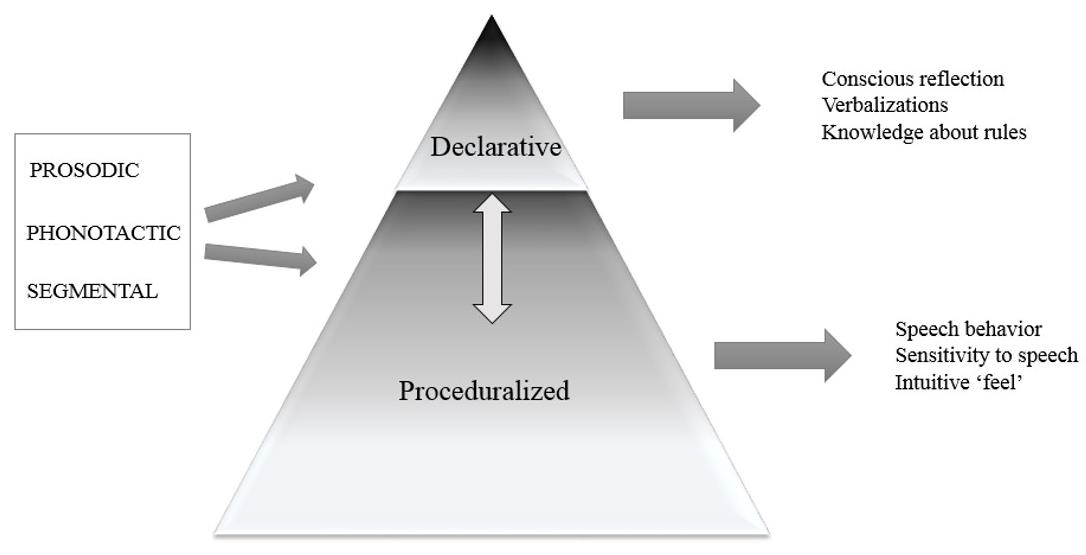
\includegraphics[width=\textwidth]{figures/a02HabilTheory-img002.png}
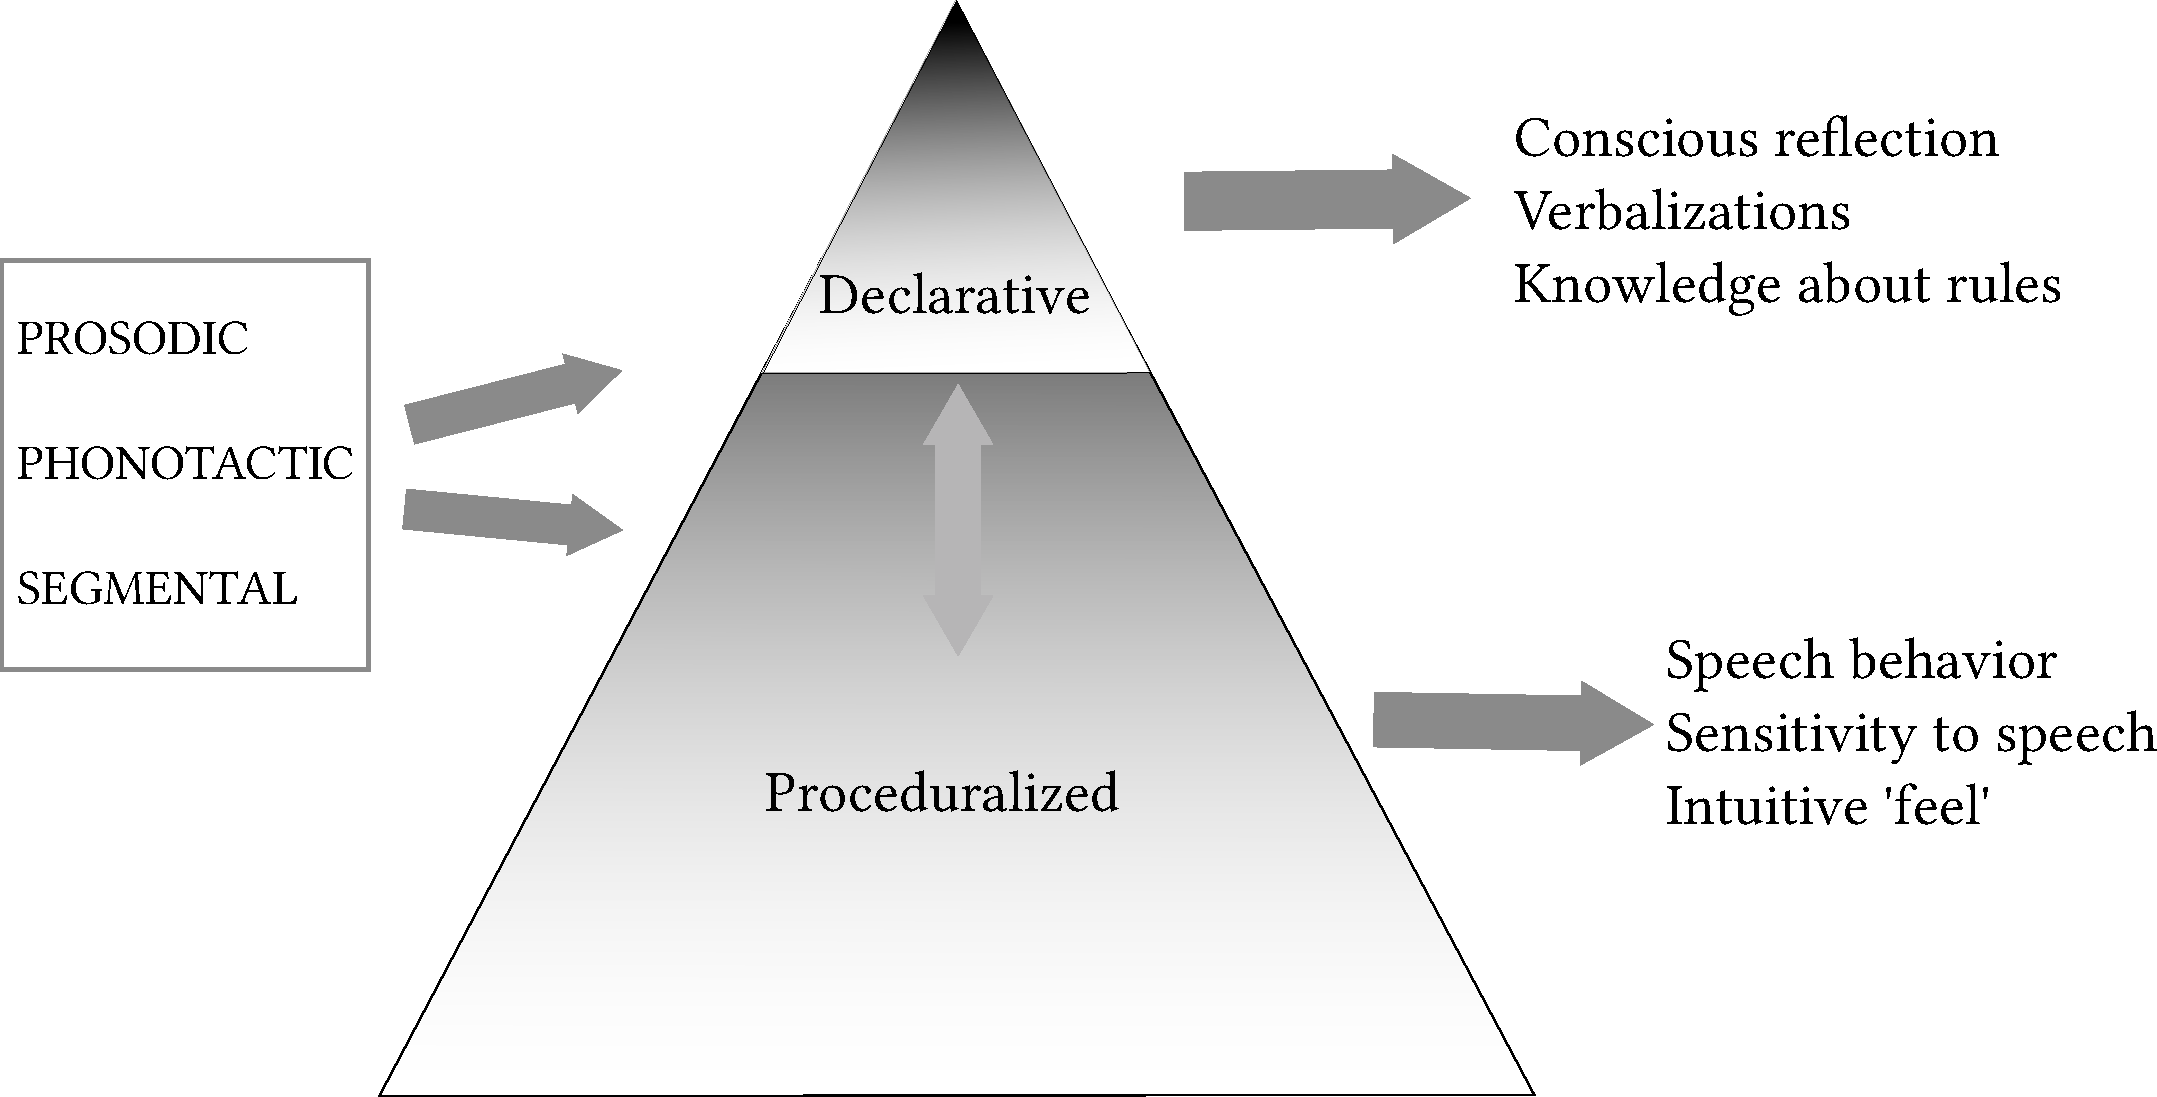
\includegraphics[width=\textwidth]{figures/a02HabilTheory-img002.pdf}
\caption{Phonological awareness in L2 according to \citet[106]{Kivistö-deSouza2015}.}
\label{fig:2.1}
\end{figure}

As already noted in the previous section, better formal instruction implies higher phonological awareness and that in turn leads to a better performance and L2 production accuracy (see, e.g., \citealt{MacKayEtAl2001, Piske2008, KennedyTrofimovich2010, Kivistö-deSouza2017}). \textit{Better} formal instruction means an explicit pronunciation instruction, involving special training in the perception and production of L2 segments as well as suprasegments.


Although the present study did not conduct any experiment in order to test and measure phonological awareness systematically across participants, the L2 learners were asked about their personal difficulties in L2 pronunciation as well as about differences between Spanish/Italian and their L1s in the semi-directed conversation conducted (see \chapref{ch:3}). The aim was to access the \textit{explicit} segmental as well as suprasegmental awareness in their L2 and to find out what sort of formal instruction they had got in terms of pronunciation. The learners were asked to answer the following two questions: \textit{What sounds or other phenomena related to pronunciation in Spanish\slash Italian differ from Czech\slash German?} and \textit{What sounds do you find difficult to pronounce or are difficult to pronounce for Czech\slash German natives in general?} Participants were helped with some words\footnote{For example, L2 Spanish learners were given the following words and expressions to get some ideas and support in this task: \textit{uno, tal, zapatos, yo, la roca, perro, un beso, vida, calles, la bodega, hombre, numeró, un agua, visión}.} and asked additional questions, if necessary. The answers obtained from this task were only supplementary; however, they allow several important observations. First, almost all the Czech speakers as well as a couple of the German speakers described Spanish/Italian pronunciation as “quite” or “(very) easy”. Not surprisingly, all the German speakers commented that the Spanish \textit{r-}sounds were the most difficult to pronounce for them or for German native speakers in general (see also \sectref{sec:2.3.1} for further details). Spanish approximants [β ð ɣ] and Italian geminate consonants were the next set of consonants they reported as being difficult.\footnote{My impression during the recordings was that most of the learners had not mastered the phonological rules of these sounds very well, but I will not go into further detail regarding the issue of explicit knowledge of these phenomena.} Second, learners showed a high sensitivity to any orthographic aspects that they felt made pronunciation confusing (e.g., <h>, <ll>, <v>). Third, most of the learners had little knowledge of articulatory phonetics, and none of them had received any specific phonetic training. In general, they had quite a limited knowledge of phonological rules in L2 and contrastive phonetics/phonology (with the exception of \textit{r-}sounds and the approximants mentioned above). Fourth, all the Czech (and some German) learners mentioned that it was very important to learn Spanish/Italian word stress placement but they did not comment on any particular difficulties with it. I assume that the Czech learners mentioned this point explicitly since Czech is a language with initial prominence and stress placement is one of the first issues that must be acquired in any L2 language with variable stress. And finally, and most importantly, none of the L2 Spanish learners mentioned anything about intonation. They were thus explicitly asked about this point and responded that they had never been trained on any aspect of L2 intonation. However, quite a different picture emerged in the L2 Italian learners. This group commented (without being explicitly asked) that the “marked”, “strong”, “melodic” or “sing-song” intonation of Italian was a very important factor for a good native-like pronunciation. The explanation may be that the “Italian melody” is more salient, musical and attractive than the Spanish one. Since they had never obtained any instructions regarding Italian intonation either, they were not able to verbalize how Italian intonation and prosody work. However, they tried to imitate, sometimes by exaggerating, its patterns intuitively by producing a larger pitch excursion and by lengthening stressed syllables (see \chapref{ch:4}).



In accordance with \citet{Kivistö-deSouza2015}, we can sum up that only a fraction of the L2 learners involved in the present study possessed \textit{declarative} (conscious) knowledge about the L2 pronunciation. Regarding intonation, the learners’ phonological awareness was found to be completely implicit or non-ver\-bal\-i\-zable, most probably because the learners had never been exposed to any explicit instruction on this topic.


\subsection{Gender}\label{sec:2.1.6} %2.1.6 /

Sociolinguistic studies usually reveal that women are important agents of advancing language change in monolingual (e.g., \citealt{Labov2001, EckertMcConnell-Ginet2003}) as well as bilingual settings (e.g.,  \citealt{LapidusShin2013}). This may be partly explained by women’s greater ability/tendency, relative to men, to “accommodate” in speech (e.g., \citealt{AsherGarcía1969, LeaperFriedman2007, Palomares2008}, see also \citealt{HancockRubin2014} for a discussion). \textit{Do women also perform differently than men in L2 speech and does gender play any role in L2 pronunciation accuracy? }Whereas some studies (e.g., \citealt{TahtaEtAl1981, Thompson1991, MunroMann2005, Hinton2013}) report that male L2 learners are rated worse for the degree of foreign accent, the majority of other studies have not found any clear difference between female and male L2 learners (e.g., \citealt{PurcellSuter1980, Elliott1995, FlegeEtAl1995, PiskeEtAl2001}). These latter studies claim that the differences are linked to other factors. In sum, the results obtained for this factor have not shown any strong enough effect of gender on degree of L2 foreign accent so far. The only difference observed between males and females is that women tend to be generally more interested in L2 learning and teaching than men. This, however, does not mean they should perform better in L2. Since previous research on gender effects has not yielded significant differences between female and male L2 learners and the number of male subjects in the present study is relatively small (see \chapref{ch:3}, \textit{\nameref{ch:3}}), this factor will not be taken into account in the present study.

\subsection{Personal and other influences}\label{sec:2.1.7}

In addition to traditionally examined factors affecting L2 speech presented in the previous sections, there is a set of further learner-external as well as learner-internal factors that may influence L2 speech. I will mention briefly some of them and start with the role of literacy and orthography in L2 speech learning. A large body of research on this issue has shown that literacy and written language shape L2 production and perception, in both positive and negative ways (see, e.g., \citealt{Rosenblum2005, PiskeEtAl2002, Bassetti2005,Bassetti2006, Bassetti2008, TaroneEtAl2013, EscuderoEtAl2014, Rafat2011,Rafat2015, Nimz2015}, among many others). These studies suggest that L2 learners tend to pronounce graphemes of L2 words as they are pronounced in their L1. For example, \citet{PeškováEtAl2017} demonstrated a negative influence of the native orthography on the duration of stressed vowels in L2 Spanish produced by L1 Czech speakers (see \sectref{sec:2.3.1.2} for details). Although we know that a specific speech style (e.g., read vs. spontaneous speech) can affect intonation patterns (see, e.g.,  \citealt{GiliFivela2008} for Pisa Italian), studies examining the influence of orthography on L2 suprasegments are still very limited in number. We also lack research that examines whether and how orthography (e.g., the use of question or exclamation marks and commas) shapes intonational patterns in L2 production. By way of exception, \citet{HeEtAl2012} showed that Chinese L2 Dutch learners tend to assign rising contours to orthographic sentences that end with a question mark and falling patterns to other sentences.


Furthermore, several studies have proved that L2 pronunciation may be positively influenced (albeit to varying extents) by personal characteristics such as motivation (e.g., \citealt{Oxford1996, BongaertsEtAl1995,BongaertsEtAl1997, Moyer1999, Dörnyei2003, DörnyeiSkehan2003, DörnyeiUshioda2011}), appropriate learning style (e.g., \citealt{Reid1995}) or extraversion (e.g., \citealt{OxfordAnderson1995}). Among other factors with a positive effect are a general talent for pronunciation (e.g., \citealt{IoupEtAl1994}) as well as aptitudes including musicality (e.g., \citealt{SlevcMiyake2006, NardoReiterer2009, MilovanovEtAl2010}), mimicry (e.g., \citealt{Hinton2013}), phonetic encoding (e.g., \citealt{HuEtAl2013}) and memory (e.g., \citealt{Carroll1990, MiyakeFriedman1998, Walter2000, WenEtAl2015, Wen2016}). Though we can anecdotally allege that some people are better “L2 pronouncers” than others, it is still not clear how such individuals’ special aptitude functions and develops.



Among all the personal factors, we can also include the strength of the (positive) attitude towards the target language and the role of (self-)identification. The present study has made several impressionistic observations about the positive relationship between a lower degree of foreign accent and the strength of acceptance of the target culture: the more speakers identify with the culture and society of the language they are learning, the better they seem to perform in the L2. For example, one female participant (24 years old), who started to teach herself Spanish at the age of 21 and moved to Spain at the age of 22, responded to a question about her native-like accent in Spanish in this way:

\begin{quote}
I think it is because I love the language so much… I can express myself even better in Spanish than in my mother tongue [Czech]. And I love Spanish people so much too; I feel like I am part of their society.
\end{quote}

Similar findings are also reported in sociolinguistic studies on positive or negative attitudes to L1 or L2 in bilingual or bidialectal communities (e.g., \citealt{Labov1972, KleeLynch2009, Silva-CorvalánEnrique-Arias2017}). A contradictory anecdote is given in \citet{DerwingMunro2015}: they describe a young Englishman living in Seville and learning Spanish under optimal conditions, who -- in spite of his rejection of his native background in favour of a new identity -- continues to speak Spanish with a rather strong English accent. Again, this illustrates the interplay among several factors affecting L2 speech acquisition, which is “beyond the speaker’s immediate control” (\citealt[29]{DerwingMunro2015}). Nevertheless, many recent studies that deal with L2 acquisition by young immigrants have shown that personal and social identity effects are very important in the process of acquiring a second language and especially its phonology (see, e.g., \citealt{Moyer2004, NortonMcKinney2011, LevisMoyer2014, Cutler2014} and works cited therein).


Another socially-related factor which has received attention in recent studies is what the literature calls \textit{accommodation} (or \textit{priming}, \textit{entrainment}) (see, e.g., \citealt{GilesEtAl1991, PickeringGarrod2004, Pardo2006, HeldnerEtAl2010, Hirschberg2011}). This process refers to the fact that we constantly adjust our way of speaking, consciously or unconsciously, according to the speech style of another participant. Our speech productions may also be “unintentionally” influenced by ambient speech, i.e., when we do not interact with anybody but just hear somebody speaking (\citealt{DelvauxSoquet2007}). Many studies on this phenomenon have proved that speakers “adapt” besides body or face gestures also features of the segmental and suprasegmental level (for a summary see \citealt[4--5]{NiebuhrMichaud2015}). Accommodation as a product of face-to-face interaction is typical also in language contact situations and plays an important role in contact-induced (in the sense used by \citealt{Trudgill1989}) phonological changes. For example, \citet{ColantoniGurlekian2004} showed by means of a prosodic analysis changes in peak alignment in “Italianized” Buenos Aires Spanish, which they attributed to three main factors: (1) historical reasons (strong Italian immigration in the 19th and 20th centuries), (2) convergence of two very similar prosodic systems (Spanish and Italian), and (3) accommodation and imitation processes. Taking into consideration that accommodation is a characteristic part of human behaviour/speech, we cannot completely exclude some kind of accommodation in the present study too. For this reason, the same person, the author, conducted all the experiments, thus ensuring that the participants were recorded under the same conditions. Whether another speaker or ambient speech could have (positively or negatively) influenced the participant directly before the experiment started was not controlled for. Furthermore, the experiment was not a face-to-face dialogue and the investigator’s interaction was held to a minimum (see \chapref{ch:3}). Other potential distracting effects such as social distance, non-native conversation or other linguistic ad-hoc convergence will have to be left outside of the present analysis.



In sum, we have seen that the majority of the factors listed above are usually investigated together with those covered in the previous sections. This is indicative of the great complexity that arises when interpreting correlations between different variables shaping an individual’s L2 pronunciation and of the necessity to treat the phenomena of L2 speech in a holistic way.


\section{Analysis of second language intonation}\label{sec:2.2}

In the previous section, we devoted our attention to core concepts of L2 speech and discussed various factors and phenomena that shape a degree of foreign accent. Since the main objective of the present empirical study is to examine intonational “errors” or interferences in L2, the intonation patterns produced in the L2 must be comprehensively described and subsequently compared with those of the respective L1s. One way to achieve this aim is to carry out linguistic analysis based on acoustic measurements and intonational transcription. In general, (linguistic) transcription can be seen as a representation of speech in written form and to some extent a kind of “simplification of reality”. Before I start to speak about a possible method for transcribing L2 intonation, it is first necessary to present some basic issues. In this section, I will begin with a definition of intonation in general and the possibilities for modelling intonation (\sectref{sec:2.2.1}), then I will present a widely used labelling system for intonation transcription called ToBI (\sectref{sec:2.2.2}) and, finally, I will describe the ToBI-based labels that will be applied to the L2 data of the present study (\sectref{sec:2.2.3}).

\subsection{Modelling of intonation patterns}\label{sec:2.2.1} %2.2.1 /

In popular speech, intonation is usually called the “melody of the language”, “a rising of a voice” or “a way of speaking”. From the linguistic perspective, intonation refers to variation of spoken pitch, of which the acoustic correlate is fundamental frequency (F0), that is, the frequency of the first harmonic (\figref{fig:2.2}).



\begin{figure}
%%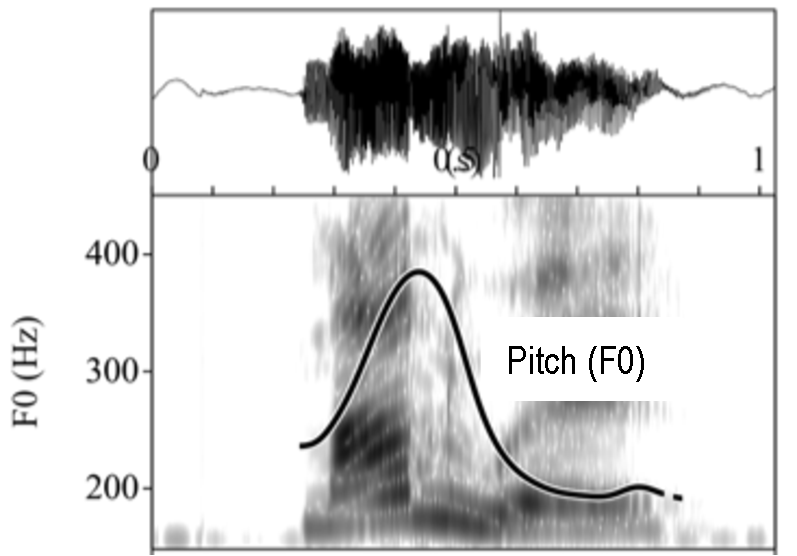
\includegraphics[width=\textwidth]{figures/a02HabilTheory-img003.emf}
%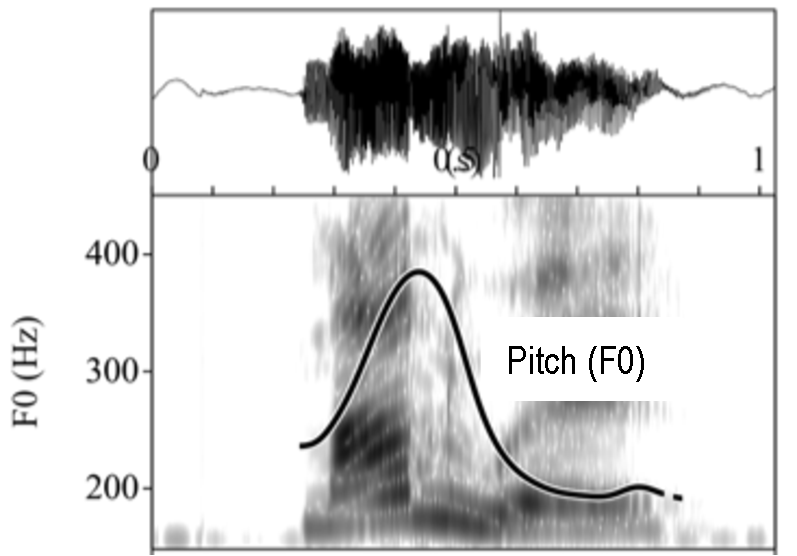
\includegraphics[width=\textwidth]{figures/a02HabilTheory-img003.pdf}
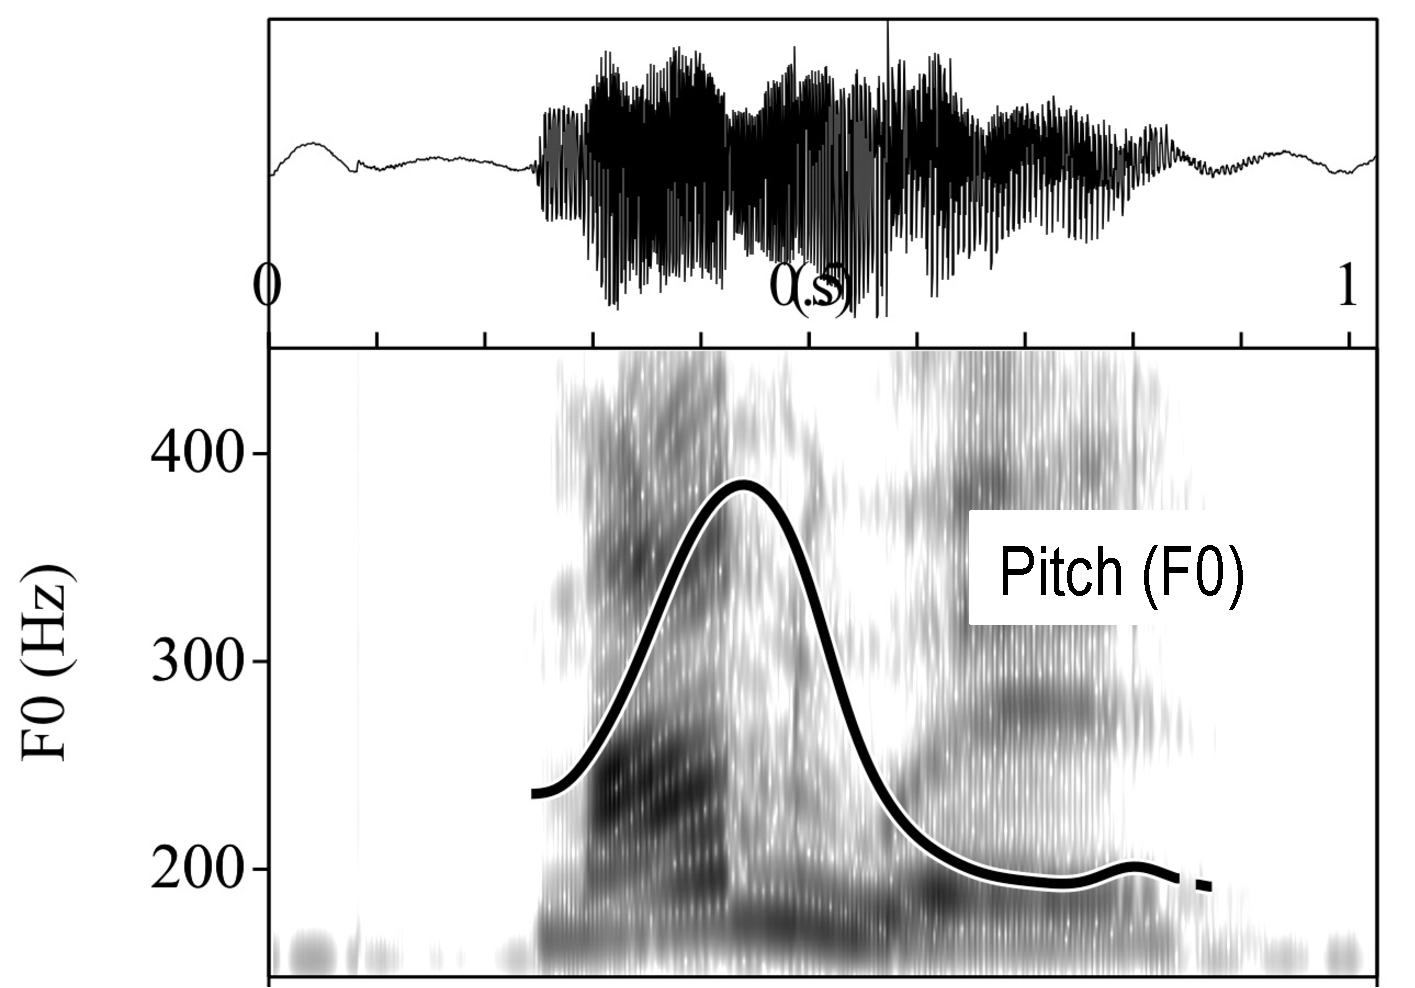
\includegraphics[width=.6\textwidth]{figures/Figure_2.2.pdf}
\caption{Track of the fundamental frequency (F0) in a spectrogram (Praat picture).}
\label{fig:2.2}
\end{figure}

However, not all uses of F0 or pitch are equivalent to intonation; for example, F0 is also used to encode lexical tonal contrasts in some languages (e.g., Mandarin Chinese) or to express paralinguistic information such as boredom or anger (see e.g. \citealt{Arvaniti2022}). More precisely, intonation is defined as the use “of \textit{suprasegmental} phonetic features to convey ‘postlexical’ or \textit{sentence-level} pragmatic meanings in \textit{a linguistically structured} way” \citep[4]{Ladd2008}. In other words, the modulation of pitch that stretches over entire utterances is not random since intonation has not only different functions but, most importantly, its own grammar within a linguistic system (e.g., \citealt{Bolinger1957, Pierrehumbert1980}). \textit{Postlexical} means that it is not determined in the lexicon, in opposite to tone (in tonal languages), stress and quantity (\citealt{HirstDiCristo1998}). Besides the grammatical or discourse and paralinguistic functions, intonation has also extralinguistic functions since it conveys information about speaker’s age, sex and further characteristics (see, e.g., \citealt[47]{Chun2002}). Furthermore, intonation is an important part of speech organisation, language’s \textit{prosody}, described as “an umbrella term that encompasses interacting phenomena that include rhythmic structure, prominence and prosodic phrasing” \citep[25]{Arvaniti2022}. I will come to the prosodic hierarchy later.


Over the last century, there have been various attempts to describe the melodic patterns of utterances in different languages and a large number of theoretical approaches to their analysis have been proposed (see, e.g., \citealt{PassyRambaud1897}, \citealt{Delattre1966} for French; \citealt{Klinghardt1923} for German;  \citealt{NavarroTomás1948}, \citealt{Quilis1975} for Spanish; \citealt{Pike1945}, \citealt{Bolinger1951,Bolinger1972a} for English; \citealt{Petřík1935a, Petřík1935b}, \citealt{Mathesius1937}, and \citealt{Daneš1957,Daneš1985} for Czech; see also \citealt{Prieto2003, Ladd2008,Ladd2015, Elvira-GarcíaEtAl2016, GiliFivelaEtAl2015, NiebuhrWard2018} for overviews on different previous and current models). However, interest in intonational research has increased very rapidly especially in the last four decades by reason of theoretical proposals on the one hand, and information technology development, on the other. Since the acoustic characteristics of intonational contours can be described and measured by means of different language technologies, “they can also be transcribed” (\citealt[768]{Elvira-GarcíaEtAl2016}). Today, there are several different systems for transcription or annotations and models of intonation (within different frameworks) available, including the IPO model (\citealt{HartEtAl1990}), the Tilt Model \citep{Taylor2000}, INTSINT \citep{HirstEtAl2000}, IViE \citep{Grabe2001}, PENTA \citep{Xu2005}, \textit{Rapid Prosody Transcription} (\citealt{ColeShattuck-Hufnagel2016}), and DIMA \citep{KüglerEtAl2015} among others. Nevertheless, one of the most popular systems for annotating intonation is ToBI, \textit{\textbf{To}nes and \textbf{B}reak \textbf{I}ndices} \citep[155]{Hualde2003}, which will also be applied in the present study (presented below). This system for the prosodic annotation of speech was introduced in 1992 for Mainstream American English (\citealt{SilvermanEtAl1992, BeckmanHirschberg1994, BeckmanEtAl2005}), but its original conventions have since been accepted and modified not only for several further English varieties but also for a large number of different languages (see, e.g., \citealt{Jun2005,Jun2014} for an overview of different ToBI systems; \citealt{BeckmanEtAl2005} for the evolution of the ToBI framework). It is important to note that ToBI is grounded in the Autosegmental-Metrical model (AM) of intonational phonology (\citealt{Pierrehumbert1980, Ladd1996}). The AM model is, as \citet[52]{Arvaniti2022} emphasizes, “fundamentally a phonological system and as such relies on the combined investigation of form and meaning” and in order to understand it, it is necessary to understand the general “organization of sound systems which recognizes both the need of abstraction and the need for phonetic detail” (see also \citealt{Arvaniti2019} for cross-linguistic variation, phonetic variability, and the formation of categories in intonation). The AM model has its roots in the British School and in studies on metrical structures and autosegments (e.g., \citealt{OConnorArnold1961, Bolinger1957, Liberman1975, Goldsmith1976, Selkirk1980}). It is called \textit{autosegmental} because the tones (T) representing the melodic part of an utterance are independent from the segments (vowels and consonants) and \textit{metrical} because they are contained in a hierarchically organised set of phonological constituents representing prominence and phrasing. These two sub-systems of (the non-linear) phonology are essential for intonation. The AM theory assumes that speech is organised in abstract, hierarchically levelled constituents, where each constituent of a lower level is enclosed within higher-level constituents. This Prosodic Hierarchy (see \citealt{Selkirk1984, NesporVogel1986/2007, Gussenhoven2002,Gussenhoven2004}, and others) with a commonly adopted set of prosodic constituents and the association of tonal events according to the AM model is depicted in \figref{fig:2.3}.




\begin{figure}
%%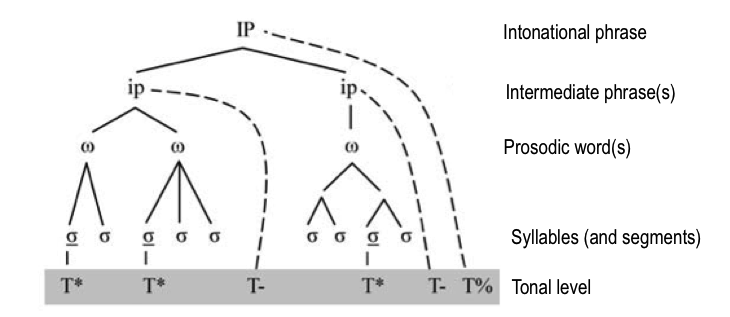
\includegraphics[width=\textwidth]{figures/a02HabilTheory-img004.png}
\begin{forest}
[IP, name = iptop, s sep=8mm
  [ip, name = ipl
    [$\omega$
      [\ul{$\sigma$}, tier=syl
        [T*, tier = word]
      ]
      [$\sigma$, tier=syl]
    ]
    [$\omega$
      [\ul{$\sigma$}, tier=syl
        [T*, tier = word, name = Tl]
      ]
      [$\sigma$, tier=syl]
      [$\sigma$, tier=syl]
    ]
  ]
  [ip, name = ipr
    [$\omega$, name=omega
      [
      [$\sigma$, tier=syl]
      [$\sigma$, tier=syl]
      ]
      [
      [\ul{$\sigma$}, tier=syl
        [T*, tier = word, name = Tr]
      ]
      [$\sigma$, name = sigma, tier=syl]
      ]
    ]
  ]
]
\node[right = 1.3cm of Tl] (T-l) {T-};
\node[right = 7mm of Tr] (T-r) {T-};
\node[right = 3mm of T-r] (T0) {T\%};
\draw[dashed] (ipl) to[out=east,in=north]  (T-l);
\draw[dashed] (ipr) to[out=east,in=north]  (T-r);
\draw[dashed] (iptop) to[out=east,in=north,looseness=1.75]  (T0);
\node[right = 2mm of T0, font=\small] {Tonal level};
\node[right = 1.9cm of sigma, font=\small, align=left] {Syllables\\(and segments)};
\node[right = 3cm of omega, font=\small] {Prosodic word(s)};
\node[right = 3cm of ipr, font=\small] {Intermediate phrase(s)};
\node[right = 5cm of iptop, font=\small] {Intonational phrase};
\end{forest}


\caption{Prosodic Hierarchy based on AM theory (adapted from \citealt[102]{GabrielEtAl2013b}).}
\label{fig:2.3}
\end{figure}

Regarding the tonal level, there are two main elements connected to different layers of the Prosodic Hierarchy: (1) tones or pitch accents which are associated with tonic syllables and marked by a star (T*), and (2) tones which signal lower, hierarchically minor or intermediate (ip) prosodic boundaries (T-) and tones which signal higher, hierarchically major or intonational (IP) prosodic boundaries (T\%).


According to \citet{Ladd1996, Ladd2008}, languages differ intonationally along the following four dimensions: (1) the \textit{semantic dimension}: languages differ in the meaning or use of the same tune (e.g., a low boundary tone can be used for a yes/no question in one language (or dialect) but not necessarily in another); (2) the \textit{systemic} \textit{dimension}: languages differ in the inventory of phonologically distinct tune types (e.g., Catalan has more contrastive tunes than Friulian, where we find more “ambiguous” tunes, see \citealt{RoseanoEtAl2015}); (3) the \textit{realisational dimension}: languages differ in the phonetic implementation of the structural elements (e.g., a rising tone in prenuclear position can be aligned with the tonic syllable in one language, whereas with the posttonic syllable in another); and (4) the \textit{phonotactic} or \textit{distributional} \textit{dimension}: languages differ in tune–text association (e.g., certain tune sequences can be associated either with the beginning or with the end of the text; \citealt[116--118]{Ladd2008}). These dimensions are crucial for the L2 Intonation Learning theory \citep{Mennen2015}, which will be presented later (see \sectref{sec:2.4.2}).


\subsection{ToBI: System for annotating intonation}\label{sec:2.2.2} %2.2.2 /

The main assumptions from the AM model outlined briefly above are also essential for understanding how the ToBI annotation system works. ToBI is an AM tool, which offers a \textit{featural} transcription in the sense that certain symbols represent basic tonal features. Some essential characteristics of the AM model will be explained here. As noted above, the transcription (or annotation) of the pitch track (F0) is based on two important tonal entities: (1) \textit{pitch accents} (PA) or tonal movements associated with the metrically strong (tonic) syllables (the stressed syllable is an important tone-bearing unit (TBU)); and (2) \textit{boundary tones} (BT) or tonal movements related to the edge of an intermediate or intonational prosodic phrase. Therefore, the name ToBI is derived from \textit{tones}, referring to pitch accents, and \textit{break}{}-\textit{indices}, indicating prosodic grouping of the words in an utterance \citep{PriceEtAl1991}. Break indices (BI) receive a number (0--4) referring to how strong the break between words or phrases is. Following general ToBI conventions, a level 0 (or BI 0) marks cohesion between orthographic words (e.g., between a phonologically dependent clitic and a lexical word, its host) that make up one prosodic word, which bears only one pitch accent (e.g., Sp. \textit{la casa} ‘the house’). BI 1 designates boundaries between two prosodic words (e.g., Sp. \textit{la casa grande} ‘the big house’). BI 2 is mostly reserved for non-phonological breaks such as hesitations.\footnote{In the case of phrase languages like French and Czech, there is a BI 2 (phonological) boundary at the edge of the accentual phrases (AP) (see \sectref{sec:2.3.2}).} In contrast to other languages like French \citep{Delais-RoussarieEtAl2015}, there is no consensus among researchers regarding level 2 in Spanish or Italian (see, e.g., \citealt{HualdePrieto2015} for Spanish;  \citealt{GiliFivelaEtAl2015} for Italian). It merely reflects a perceived disjuncture with no intonational effect, and no slowing or other break cues. A level 3 is assigned at the edge of the Intermediate Phrase (ip), which is dominated by the BI 4, the Intonational Phrase (IP) corresponding to the end of main prosodic units (see \citealt{FrotaEtAl2007} for prosodic phrasing in different Romance languages).


These specified tonal targets (PA and BT) are the most important units, where\-as the rest of the contour is formed by phonetic interpolation between them, which is not phonological. The last pitch accent before any ip or IP boundary is called a nuclear accent, whereas the preceding pitch accents are counted as prenuclear pitch accents. ToBI operates with two basic tone levels and their possible combinations, a high tone (H) versus a low tone (L) in the local pitch range. The high targets are not obligatorily aligned with the tonic syllables; the tonal peak of the pitch accent can be reached, for instance, at the end of the posttonic syllable. For such cases, ToBI uses further diacritics for additional information. The alignment for the late peak is tagged with the symbol ``<'' (this is used when the H tone is aligned with the posttonic syllable). Furthermore, ToBI uses the tags ``!'' for downstep (when the pitch of a tonal unit is lower than the pitch of the preceding tone) and ``¡'' for upstep (when the pitch of a tonal unit is higher than the pitch of a preceding tone or its pitch range is wider). We usually do not transcribe a \textit{downstep} (!H) when it is predictable, for example, by the declination in statements, but we always do transcribe an \textit{upstep} (¡H). The diacritics are used for refining phonetic differences between tonal units, or, phonologically, when two entities stand in contrast, that is, when speakers associate the tones with two different meanings. Further details on labelling applied in this study will be presented in \chapref{ch:3}.



Although ToBI is designed to be language-specific and several ToBI annotation systems for different languages have already been proposed (e.g., GToBI for German, Sp\_ToBI for Spanish, Cat\_ToBI for Catalan, K-ToBI for Korean), there is also a set of community-wide conventions adopted by all ToBI users. First of all, the analysis of phonetic evidence must be based on both auditory perception and visual examination of the F0 curve by means of a specific program for phonetic analysis of speech (e.g., Praat). Next, it is univocal: for example, a high tone is always transcribed as H(igh) and H cannot be used for another entity. ToBI labellers thus agree to adopt the same labels and to maintain consistency (which does not mean that changes are prohibited). And finally, it is “easy to teach” and “accessible to a fairly wide audience, without assuming any background in linguistics or speech sciences” (see English ToBI at \url{https://www.ling.ohio-state.edu/~tobi/} and Spanish ToBI at \url{http://prosodia.upf.edu/sp\_ tobi/en/index.php}). While it is true that ToBI is easy to learn and understand, its simplicity and practical application to data are not unproblematic and ToBI annotation implies several important requirements. Initially, a labeller must have \textit{a priori} knowledge of the language under study and above all its phonology, must be familiar with (acoustic) phonetics, and must possess advanced user skills for Praat (or any other similar program), in order to avoid software errors and prevent micro-prosody effects from shaping the pitch contour. In addition, the labeller must be able not only to read the shape of F0 contours but also to understand how prosody functions to mark grammatical contrasts in that language (see, e.g., \citealt{Arvaniti2016}) because tonal targets have a linguistic meaning and important function in phonological, morphological, semantic, pragmatic, and even sociolinguistic contexts (\citealt{JunFletcher2014}). The perception factor should not be underestimated either; some researchers even suggest a “Label what you hear” guideline \citep[28]{Wightman2002}, which should take precedence over the description of the shape of the pitch track (for a similar view see \citealt{Romportl2008}). Notwithstanding, practice has shown that even trained and experienced labellers may still diverge in the way they interpret and transcribe intonational curves. Prosodic annotation is thus challenging for a number of factors, among which \citet{ColeShattuck-Hufnagel2016} list speech rate, style, nuances of pragmatic meanings, reduced or ambiguous acoustic cues as well as influence from the linguistic context. One of the principal difficulties is the potential for differing and subjective interpretations of the phonetic-phonology interface, presupposing the existence of discrete entities (i.e., tones). ToBI is primarily phonological because it shares basic assumptions from AM, which relies on an abstract phonological representation connected with pitch contours, considering intonation an important part of a language’s grammar. However, we often find inconsistencies and phonetic-like instead of phonemic transcription in the studies applying ToBI. Typical sources of confusion for labellers in tagging processes are the transcription of truncated pitch contours, reductions in the acoustic signal, tonal clashes, contrasts of alignment, indications of downstep/upstep, and many other phenomena (\citealt{ColeShattuck-Hufnagel2016, JunEtAl2015, HualdePrieto2016}). Therefore, the introduction of two levels of representation in a prosodic annotation can be a very good solution here: “One, phonological, where meaningless (and predictable) variation in alignment and range is ignored and another, broad phonetic, where these differences are represented” (\citealt[15]{HualdePrieto2016}). According to \citet{HualdePrieto2016}, this can make it easier to understand tonal contrasts in a cross-linguistic perspective but most importantly within one language (for a critical view on broad phonetic transcription, see \citealt{Arvaniti2016,Arvaniti2022, CangemiGrice2016, ColeShattuck-Hufnagel2016}). For example, vocative chants in Catalan have one phonological underlying tone /L+H* !H\%/ with two possible phonetic realizations: [L+H* !H\%] and [H* !H\%] depending on the context (\citealt[13--14]{HualdePrieto2016}). The [L+H* !H\%] variant is phonetically realized as a rise and the [H* !H\%] as a high plateau (H) during the tonic syllable. Both nuclear accents are followed by a sustained mid level plateau (!H). The two allotones are in complementary distribution: If the word begins with an unaccented syllable (e.g., \textit{Ma}\textbf{\textit{ri}}\textit{na!}), the low tone (L) is phonetically realized on the surface (L+H*). On the other hand, if the word begins with an accented syllable and a voiceless plosive (\textbf{\textit{Pau}}\textit{la!}), the L tone is not expressed overtly (H*) (\figref{fig:2.4}).




\begin{figure}
%%\includegraphics[width=\textwidth]{figures/a02HabilTheory-img005.tif}
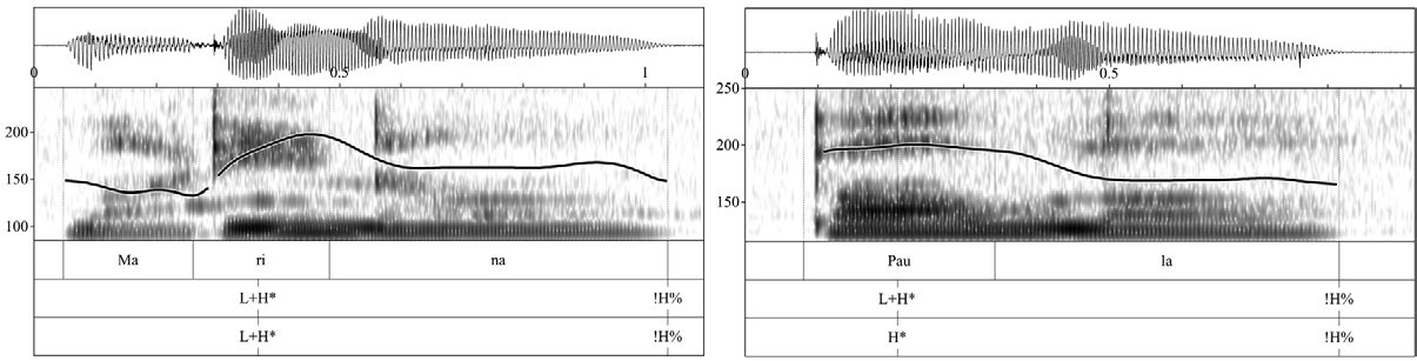
\includegraphics[width=\textwidth]{figures/a02HabilTheory-img005-new.png}


\caption{Phonological (second tier) and broad phonetic (third tier) representations of the vocative chant in Catalan (taken from \citealt[14]{HualdePrieto2016}).}
\label{fig:2.4}
\end{figure}


The treatment of the phonetic-phonology interface, presenting also a notorious degree of variability across speakers and contexts, is still a widely debated and challenging issue in intonational research (see, e.g., \citealt{Wightman2002, BreenEtAl2012, ColeEtAl2014, ColeShattuck-Hufnagel2016, Pešková2018}).



In sum, the ToBI approach has received many criticisms: it is said to be too phonetic, it is too phonological, it is too subjective, it is not applicable to all languages, etc. In my opinion, in spite of these various (and important) critical points, ToBI can be seen as a useful approach for the description and systematization of intonation patterns and “as a tool for testing and evaluating hypotheses to improve the intonation model” (\citealt[518]{JunFletcher2014}). Moreover, several studies have shown by means of intertranscriber reliability tests a high degree of agreement or consistency among trained labellers thus proving the functional utility of ToBI for prosodic annotation (see, e.g., \citealt{PitrelliEtAl1994, YoonEtAl2004, EscuderoEtAl2012, MennenEtAl2012, Feldhausen2016, Elvira-GarcíaEtAl2016}).


\subsection{Application of ToBI labels on L2 data of the present study}\label{sec:2.2.3} %2.2.3 /
\begin{sloppypar}
As the present study deals with L2 intonation contours, here the question emerges: ToBI, or not ToBI? I have decided for a ToBI non-language-specific and phonetic-based labelling in order to provide simplified representations of tonal events, on the one hand, and to systematize and compare the patterns found in data, on the other hand. The aim of the phonetically transparent analysis here is to detect and compare differences between the L1 and L2 systems and to explain non-native productions. The idea of non-language-specific labels is not new and ToBI or AM-based labels for L2 intonation (with modifications or deviations) have already been used in different studies on L2 intonation (e.g., \citealt{JunOh2000, MennenEtAl2012, Mennen2015, AstrucVanrell2016, ColantoniEtAl2016a}, and many others). This annotation with phonetic labels is indirectly in line with the recent -- but so far not overall accepted -- proposal for the development of the \textit{International Prosodic Alphabet} (IPrA) that offers “a set of cross-linguistically transparent and consistent labels” based on ToBI annotation (\citealt[1]{HualdePrieto2016}). According to the authors of this proposal, “the IPrA tool can be useful for L2 prosodic studies […], as right now it is difficult to transcribe L2 speech when working with two established ToBI systems” (\citealt[19]{HualdePrieto2016}, see also \citealt{JunFletcher2014}). A similar view was taken by the authors of the Eti\_ToBI automatic intonation transcriber for Spanish (\textit{El etiquetador ToBI}, \citealt{Elvira-GarcíaEtAl2016}), who argue that “a standard (non-language related) ToBI method for analysing prosody is possible” since it “provides an objective, transparent and universal transcription based only on acoustic data” (\citealt[785]{Elvira-GarcíaEtAl2016}) (see \sectref{sec:3.4.1}). The present study applies or modifies for its purposes these two projects and available AM transcription systems for the languages under study. The following inventory of nuclear pitch accents and boundary tones (ip/IP) proved to be important for the data of the present study (see Figures \ref{fig:2.5}--\ref{fig:2.6} for a schematic representation of the F0 track and Tables~\ref{tab:2.4a}--\ref{tab:2.4b} for a phonetic description of the tonal events). The tonal inventories of the languages under study are presented in \sectref{sec:2.3.2}. We will see examples of these patterns later in Chapters~\ref{ch:3} and \ref{ch:4}.
\end{sloppypar}


\begin{figure}
%%\includegraphics[width=\textwidth]{figures/a02HabilTheory-img006.emf}
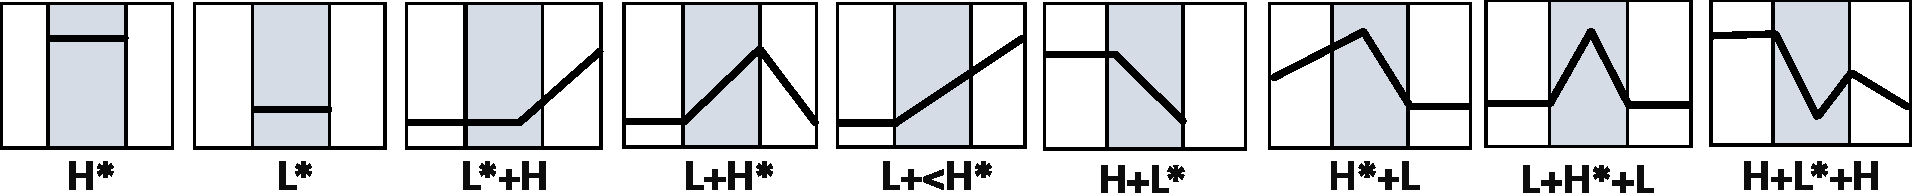
\includegraphics[width=\textwidth]{figures/a02HabilTheory-img006.pdf}
\caption{Schematic representation of pitch accents found in both L1 and L2 data.}
\label{fig:2.5}
\end{figure}

\begin{figure}
%%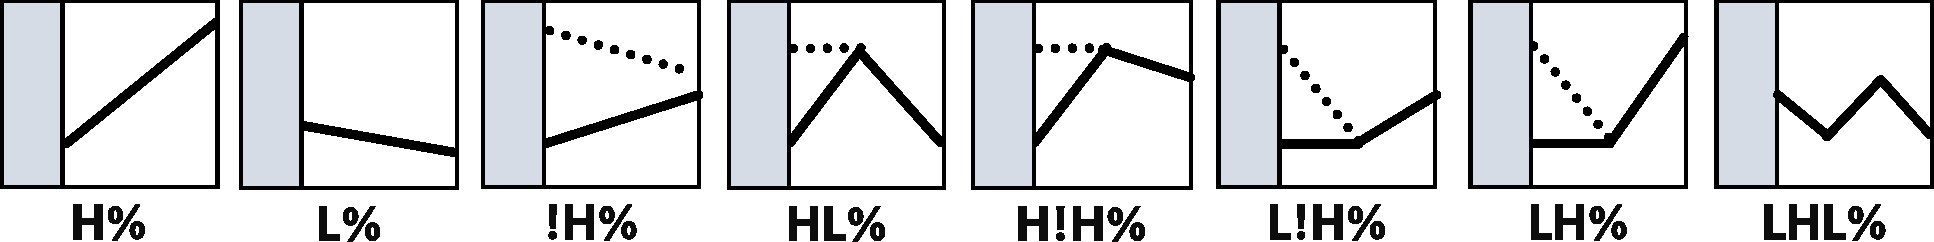
\includegraphics[width=\textwidth]{figures/a02HabilTheory-img007.emf}
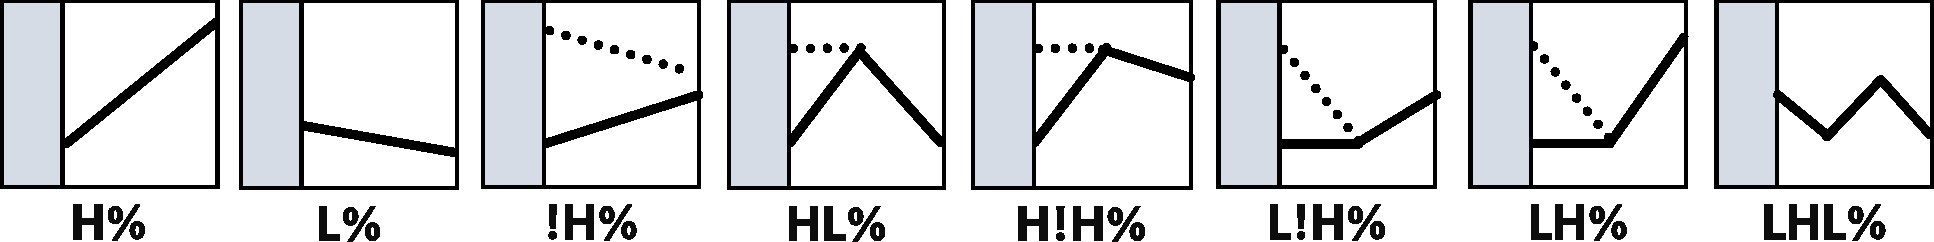
\includegraphics[width=.8\textwidth]{figures/a02HabilTheory-img007.pdf}
\caption{Schematic representation of boundary tones found in the data (the dotted line indicates alternative pitch tracks).}
\label{fig:2.6}
\end{figure}

\begin{table}
\begin{tabularx}{\textwidth}{p{3cm}Q}
\lsptoprule
Tonal entity & Description of the phonetic realization\\\midrule
H* & High plateau without any preceding F0 valley.\\
\tablevspace
L* & Low plateau at the low level of the speaker’s range.\\
\tablevspace
L*+H & Low plateau in the tonic syllable, which is followed by a rising F0 movement in the posttonic syllable.\\
\tablevspace
L+H* & Rising F0 movement during the tonic syllable with the F0 peak located at its end.\\
\tablevspace
L+<H* & Rising F0 movement during the tonic syllable with its F0 peak aligned with the posttonic syllable.\\
\tablevspace
H+L* & F0 fall within the temporal limits of the tonic syllable (with a high target in the pretonic syllable).\\
\tablevspace
H*+L & F0 rising pattern at the beginning and a falling pattern in the tonic syllable. The fall is dominant. \\
\tablevspace
L+H*+L

(L+H* or H*+L in Italian ToBI) & Balanced rising-falling pattern located within the tonic syllable.\\
\tablevspace
H+L*+H

(L*+>H in Italian ToBI) & Falling-rising pattern within the tonic syllable. The start of the fall is (roughly) aligned with the beginning of the tonic syllable. The rise is always smaller than the fall; both occur in the tonic syllable.\\
\lspbottomrule
\end{tabularx}
\caption{Inventory and description of prenuclear and nuclear pitch accents used in the present study. The phonetic description of these tonal representations is based on \citet{AguilarEtAl2009}, \citet{Estebas-VilaplanaPrieto2008}, \citet{GabrielEtAl2010} and  \citet{GiliFivelaEtAl2015}.\label{tab:2.4a}}
\end{table}


\begin{table}
\caption{Inventory and description of boundary tones (ip, IP) used in the present study. The phonetic description of these tonal representations is based on \citet{AguilarEtAl2009}, \citet{Estebas-VilaplanaPrieto2008}, \citet{GabrielEtAl2010} and  \citet{GiliFivelaEtAl2015}.\label{tab:2.4b}}
\begin{tabularx}{\textwidth}{lQ}
\lsptoprule
{Tonal entity} & {Description of the phonetic realization}\\
\midrule
H-, H\% & Rising F0 movement after a H or L pitch accent.\\
\tablevspace
L-, L\% & Low sustained or falling tone at the speaker’s baseline.\\
\tablevspace
!H-, !H\% & Slightly rising or falling F0 movement towards a middle target (also called “sustained” pitch).\\
\tablevspace
HL-, HL\% & F0 peak with a subsequent fall.\\
\tablevspace
H!H-, H!H\% & F0 peak with a slight fall towards a middle target.\\
\tablevspace
L!H-, L!H\% & Low sustained tone followed by a slightly rising F0 movement towards a middle target.\\
\tablevspace
LH-, LH\% & Low sustained tone followed by a sharp rising F0 movement.\\
\tablevspace
LHL-, LHL\% & Complex pitch movement consisting of a fall plus rise and then a fall to a low F0 value. (This pattern is attested only in L1 Spanish in exhortative requests.)\\
\tablevspace
Hi & Initial pitch (sometimes transcribed as \%H). This high tone marks a phrase at the beginning of the speaker’s pitch range and is not attributed to the first pitch accent of the utterance. It was transcribed only if it was articulated as a high plateau which could not be attributed to a high pitch accent (H*); this was the case when the first word of an utterance begins with an unaccented syllable. \\
\lspbottomrule
\end{tabularx}
\end{table}


In general, there are no major differences between the labels used here and those applied in previous work. However, the present study differs with regard to the treatment of tritonal pitch accents. In comparison to the IPrA and the ToBI systems, which usually do not account for tritonal realizations of pitch accents, the present work includes two tritonal pitch accents (H+L*+H, L+H*+L) in its analysis. The H+L*+H tone reported here is similar to an IPrA H+!H* tone, but they are not identical: H+L*+H has a sharp fall and a moderate rise to a mid level, whereas a H+!H* has a falling pattern to a mid level.\footnote{The H+!H* tone has been documented, for example, in German \citep{GriceEtAl2005a} and French \citep{Delais-RoussarieEtAl2015}. It is very similar to H+L*, a label which is used here.}  It corresponds to the Italian L*+>H in  \citet{GiliFivelaEtAl2015}, but the label H+L*+H is preferred here in order to specify the exact tritonal F0 movement within the stressed syllable. As for L+H*+L, it has an equilibrated rising-falling pattern located within the tonic syllable (mostly the tonic vowel) and it is thus realized and perceived differently from H*+L, H+L* or L+H*. The tag L+H*+L has been proposed for Pisa Italian (\citealt{GiliFivela2002,GiliFivela2004, PrietoEtAl2005}) as well as Argentinean Spanish (an “Italianized” variety of Spanish, see, e.g., \citealt{GabrielEtAl2010, GabrielKireva2014a}). Production and perception experiments motivated the assumption that L+H*+L is the phonological nuclear accent for expressing focus, contrast or emphasis in Argentinean Spanish (see, e.g., \citealt{GabrielEtAl2010, FeldhausenEtAl2011}). In Italian, a tritonal pattern as an underlying category has not been fully accepted:  \citet[148]{GiliFivelaEtAl2015} point out that the pattern with a tritonal shape within the stressed syllable belongs to the underlying ``early-peak'' (L+H*) pattern or H*+L depending from L1 Italian varieties (see, for instance, nuclear pitch accents in their examples in Fig. 5.5, pg. 162; see also  \citealt{GiliFivela2002,GiliFivela2004} for further details).\footnote{L+H*+L is regarded as a phonetic variant of the phonological pattern /H*+L/ by \citet{GiliFivela2002, GiliFivela2004}, who leaves the leading tone [L] merely for phonetic purposes because the trailing pattern is sufficient for phonological contrast.}


The following section presents phonological systems of the languages under study, including their segmental and suprasegmental features.


\section{Phonological systems of the languages under study}\label{sec:2.3}

The objective of this section is to present and compare the main segmental and suprasegmental properties of the languages under study. Since foreign accent is a typical feature of L2 speech and articulation of segments plays an important role in it, first, segmental dissimilarities and similarities across the languages under study are considered (\sectref{sec:2.3.1}). Next, the main suprasegmental characteristics, including rhythm, stress and intonation, together with the prosodic typology of the languages are presented (\sectref{sec:2.3.2}).

\subsection{Segmental inventories in contrast}\label{sec:2.3.1} %2.3.1 /

The comparison of the systems predicts where the learners might have major problems with target-like pronunciation and according to which -- potentially transferred -- vowels and consonants we might be able to distinguish a German L2 learner from a Czech L2 learner. Given the fact that segments are not the main focus of this study, I will present only the most important phenomena, without going into a detailed discussion on dialectal differences or factors such as speaking style. The summary in \tabref{tab:2.5a} is based on the following literature: \citet{Canepari1992}, \citet{RogersdArcangeli2004}, \citet{LoporcaroBertinetto2005} for Italian; \citet{Hualde2005, Hualde2014}, \citet{GabrielEtAl2013a} for Spanish; \citet{Palková1994}, \citet{Dankovičová1999}, \citet{Volín2010}, \citet{ŠimáckováEtAl2012}, \citet{SkarnitzlEtAl2016} for Czech; \citet{Kohler1995, Kohler1990, Kohler1999}, \citet{Mangold2005}, \citet{Hall2011}, \citet{MeibauerEtAl2015} for German. Some transferred phenomena will be illustrated by means of the L2 data collected in the production experiment of the present study (see \chapref{ch:3}).

\begin{sidewaystable}

\begin{tabularx}{\textwidth}{QQQQQ}

\lsptoprule

{Segmental} & \multicolumn{2}{l}{{Target languages}} & \multicolumn{2}{l}{{L1 backgrounds}}\\
\cmidrule(lr){2-3}\cmidrule(lr){4-5}
Features & {Italian} & {Spanish} & {Czech} & {German}\\
\midrule
Vowel quality & / a e ɛ i o ɔ u / & / a e i o u / & / a ɛ ɪ o u

aː ɛː iː oː uː / & / i y ɪ ʏ e ø ɛ œ ə ɐ a ɑ ɔ o ʊ u / \\
\tablevspace
Vowel quantity & No phonemic opposition

(but stressed open vowels are longer) & No phonemic opposition & Phonemic opposition & Phonemic opposition only in stressed syllables\\
\tablevspace
Vowel reduction & No & No & No & Yes \\
\tablevspace
Consonant quantity & Geminates & No geminates & No geminates & No geminates\\
\tablevspace
VOT / p t k / & Zero VOT & Zero VOT & Zero VOT & Positive VOT

(aspiration)\\
\tablevspace
VOT / b d ɡ / & Negative VOT & Negative VOT & Negative VOT & Zero VOT\footnote{For a better comparison, I use the term ``zero VOT'' (e.g., \citealt{RakowLleó2008}), although voiceless plosives show a certain degree of positive VOT and ``devoicing'' \citep[58]{Catford1988} might be an alternative term here.}\\
\tablevspace
Pronunciation of

/ b d ɡ / & Plosive & Plosive or Approximant

[β ð ɣ] & Plosive & Plosive\\
\midrule
\end{tabularx}
\caption{Main segmental features of Italian, Spanish, Czech and German in contrast.}
\label{tab:2.5a}
\end{sidewaystable}
\begin{sidewaystable}\ContinuedFloat

\begin{tabularx}{\textwidth}{QQQQQ}

\midrule

{Segmental} & \multicolumn{2}{l}{{Target languages}} & \multicolumn{2}{l}{{L1 backgrounds}}\\
\cmidrule(lr){2-3}\cmidrule(lr){4-5}
Features & {Italian} & {Spanish} & {Czech} & {German}\\
\midrule
Final-obstruent devoicing & No & No & Yes & Yes\\
\tablevspace
Pronunciation of rhotics & [r] & [r], [ɾ] & [r] & [ʁ], usually vocalized in coda position\\
\tablevspace
Pronunciation of laterals & “light” /l/ & “light” /l/ & velarized or “dark” /l/ & “light” /l/\\
\tablevspace
Further potential difficulties for L2 learners & [ʎ] & [ʎ], [θ], [ʝ] & -- & --\\
\tablevspace
Syllable structure\footnote{See WALS \citep{Maddieson2013} for the terms used here.} & Moderately complex syllable structure & Moderately complex syllable structure & Complex syllable structure & Complex syllable structure\\
\tablevspace
C\#V sequences & Resyllabification & Resyllabification & Optional resyllabification; optional assertion of glottal stop before initial vowels & No resyllabification; assertion of glottal stop before initial vowels\\
\lspbottomrule
\end{tabularx}


%\caption{Main segmental features of Italian, Spanish, Czech and German in contrast (continued).}
%\label{tab:2.5b}
\end{sidewaystable}

\subsubsection{Vowels}\label{sec:2.3.1.1}

First of all, we observe that the two Romance languages display quite a limited vowel system. Both have no phonemic opposition in duration, although traditionally it has been claimed that in Italian vowels in stressed open syllables have longer duration than unstressed vowels or vowels in closed syllables. Against this traditional phonetic approach, however, \citet{DImperioRosenthall1999} have proved that the increased duration is not equal in all positions and have proposed that the lengthening of penultimate syllables is phonological. In contrast, Czech is a typical quantity language in that it differentiates phonologically between short and long vowels, the durational ratio between them being about 1:1.3--1.8 depending on the vowel (\citealt[51]{SkarnitzlEtAl2016}). The durational opposition is allowed in both stressed and unstressed positions in Czech (e.g., [ˈmɪ.laː], ‘kind-\textsc{f}’ vs. [ˈmɪ.la] ‘she washed’). In this respect, Czech differs substantially from the other languages, in which unstressed vowels cannot be longer than stressed vowels (with the exception of final/preboundary syllables, which are intrinsically longer) (see also \sectref{sec:2.3.2}). This is also why many non-native speakers may perceive unstressed syllables with a long vowel as stressed syllables in Czech (e.g., \textit{Janáček} [ˈjanaːtʃɛk], perceived as [jaˈnaːtʃɛk]). Notice that a long vowel is orthographically marked with an acute accent in Czech. Due to the similarities in vowel quality, Czech learners have no special difficulties with the acquisition of the Italian or Spanish vowel systems. The only problem that can arise is with the opposition of /e/ vs. /ɛ/ and /o/ vs. /ɔ/ in Italian. German has the most complex vowel quality system, displaying also durational opposition, which is restricted to stressed syllables. Additionally, it reduces or deletes vowels in unstressed positions; this property is very often transferred to an L2. For example, the unstressed vowel /o/ in the Spanish word \textit{perro} ‘dog’ is usually pronounced in a very close-mid manner, what natives might perceive as something like [u].\pagebreak

\subsubsection{Consonants}\label{sec:2.3.1.2}

Regarding the pronunciation of consonants, every language shows its own particularities. Italian is a language that geminates consonants, a property causing difficulties for many L2 learners who do not have this feature in their phonological systems. Spanish is the only language that displays approximant allophones [β ð ɣ] of the voiced plosives in specific contexts, and this is where many L2 learners show articulation difficulties even at a very advanced level. In contrast, German is the only language that -- under certain conditions -- aspirates voiceless stop consonants and has zero VOT in the case of voiced stops, meaning that there is (almost) no voicing at the instant of the articulation closure. This is why native hearers tend to interpret German learners’ [b d ɡ] as [p t k] (e.g., the Spanish word \textit{drama} ‘drama’ may sound like \textit{trama} ‘plot’). \figref{fig:2.7} offers an example of an aspirated /t/ in L2 Spanish as produced by an L1 German learner.\footnote{I applied the figure-drawing Praat script by \citet{Elvira-García2014} to generate all Praat figures in the text.} Notice that the intervocalic /b/ was not produced as an approximant [β] in accordance with the rules of Spanish phonology.


\vfill
\begin{figure}[H]
%%\includegraphics[width=\textwidth]{figures/a02HabilTheory-img008.tif}
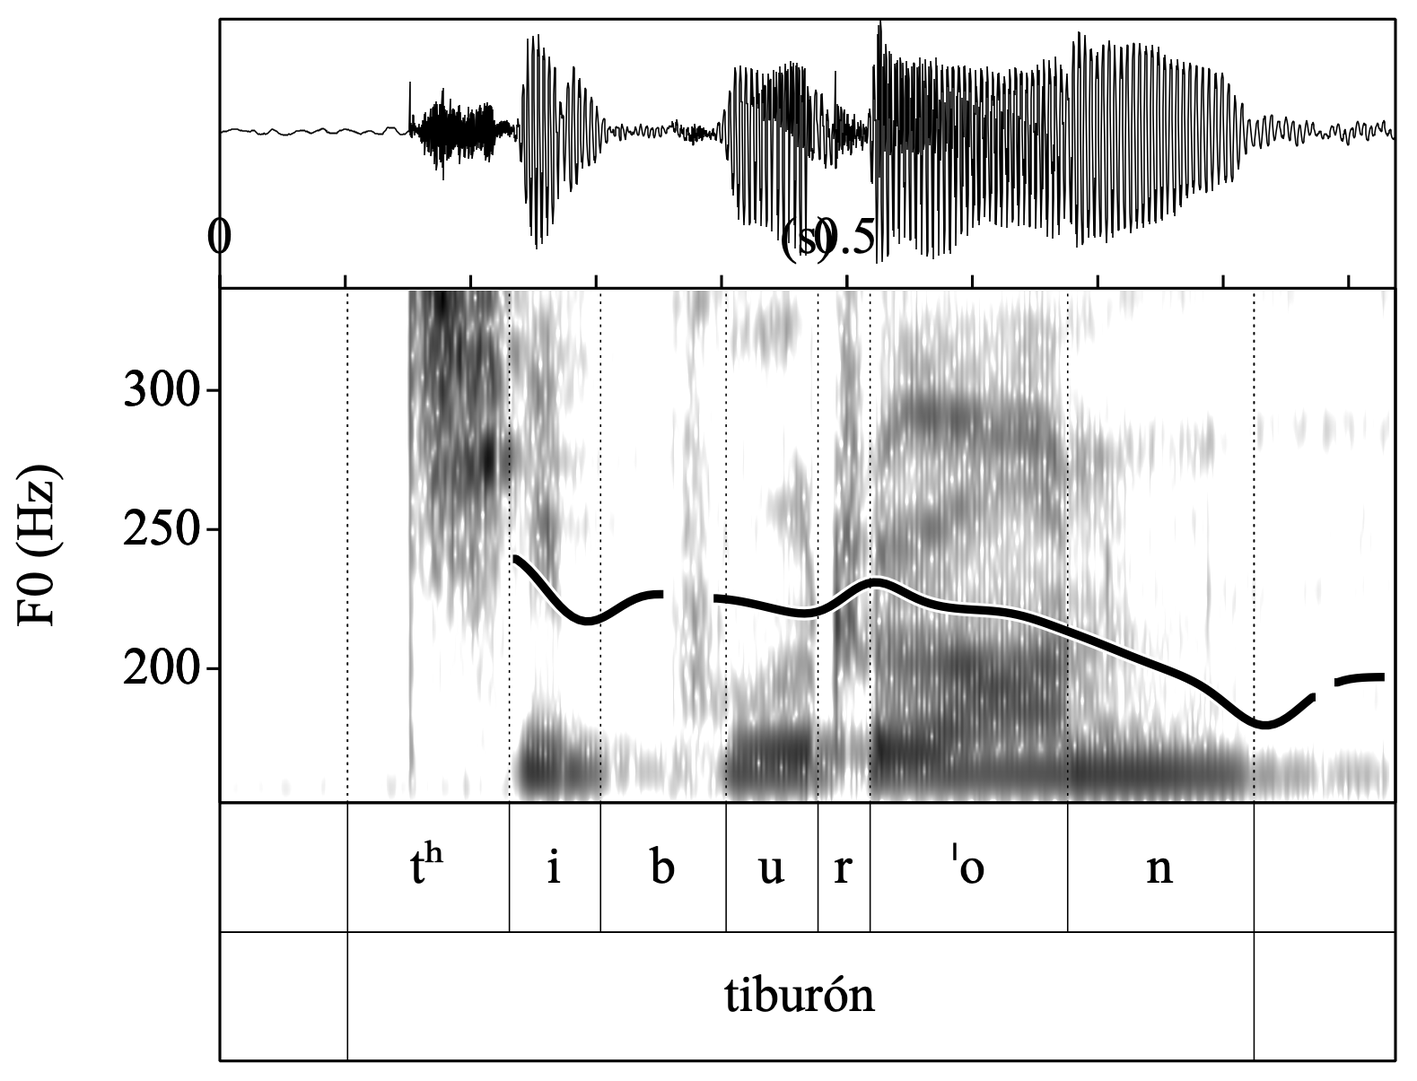
\includegraphics[width=.7\textwidth]{figures/a02HabilTheory-img008-new.png}
\caption{Aspiration of /t/ in the word \textit{tiburón} ‘shark’ in L2 Spanish produced by an L1 German learner (F\_19).}
\label{fig:2.7}
\end{figure}
\vfill\pagebreak


In contrast to Italian and Spanish, German and Czech show final-obstruent devoicing, which can be observed in L2 as well (\figref{fig:2.8}).\footnote{The correct pronunciation of the final consonant in this position in Spanish would be [\textrm{baɾ.βa.ɾi.ˈðað}], [\textrm{baɾ.βa.ɾi.ˈða}\textrm{\textsuperscript{ð}}], [\textrm{baɾ.βa.ɾi.ˈða}] or [\textrm{baɾ.βa.ɾi.ˈðaθ}], depending on the speech style and/or dialect. In Italian, the voiced obstruent is maintained in such cases (e.g., <sud> [\textrm{ˈsud}], ‘south’).}



\begin{figure}
%%\includegraphics[width=\textwidth]{figures/a02HabilTheory-img009.tif}
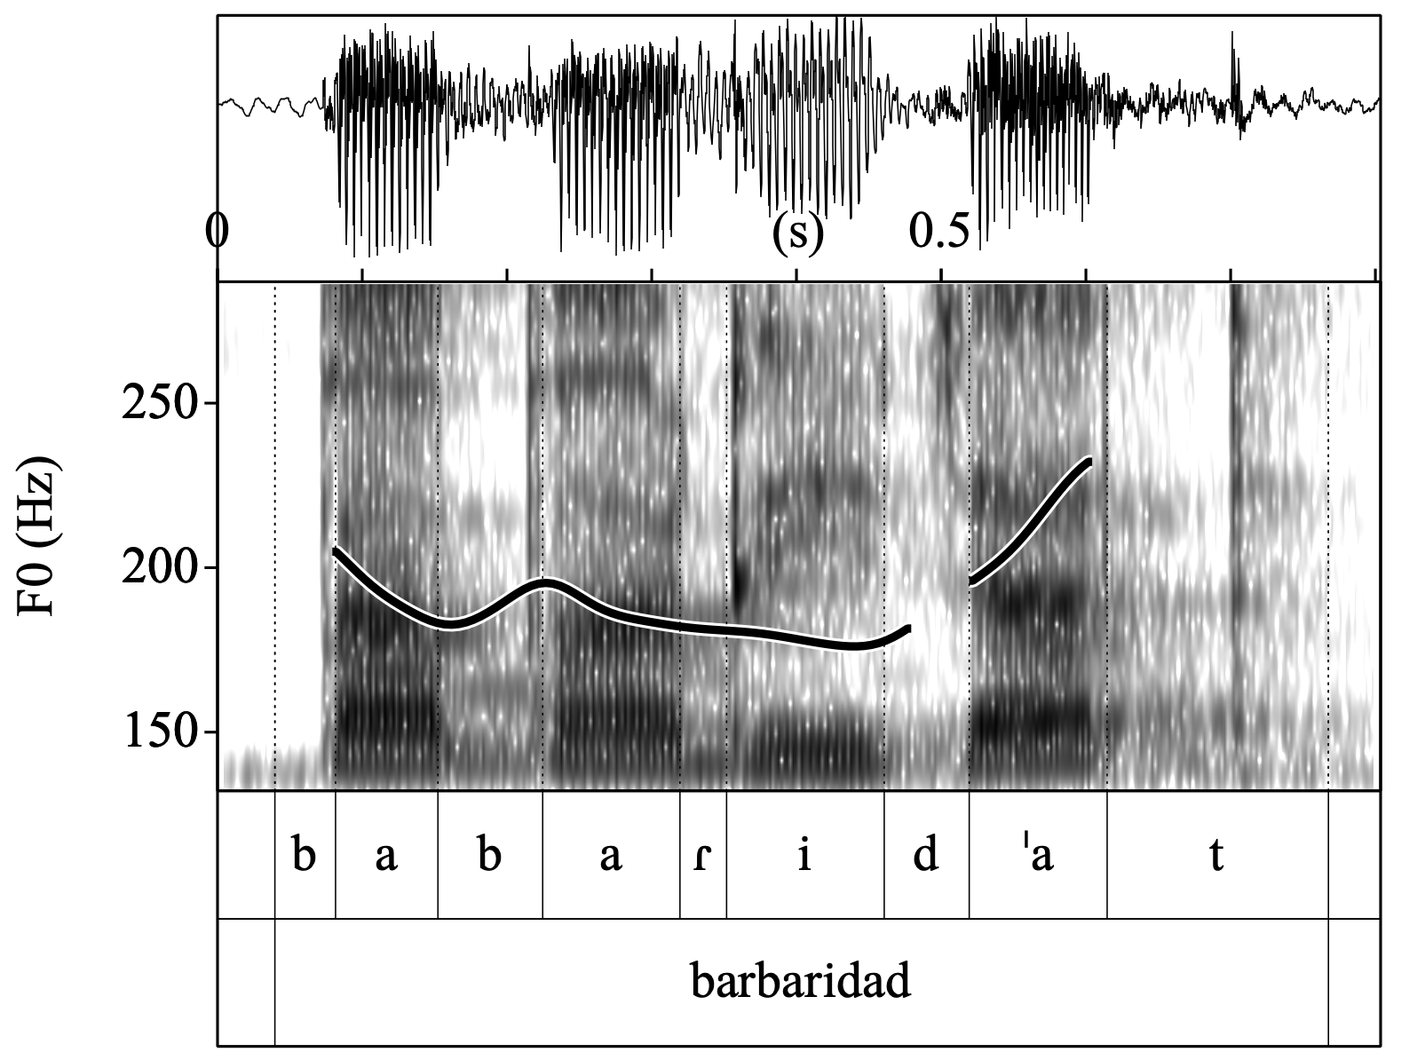
\includegraphics[width=.7\textwidth]{figures/a02HabilTheory-img009-new.png}



\caption{Final-obstruent devoicing of /d/ in the word \textit{barbaridad} (‘barbarity’) in L2 Spanish produced by an L1 German learner (F\_06).}
\label{fig:2.8}
\end{figure}


It is well known that the pronunciation of Spanish rhotics causes the most difficulty for German learners, who do not have this sound in their L1 consonant inventory. Thus, German learners can be easily identified by the mispronunciation of the rhotics (trill and tap), together with the aspiration of voiceless stop consonants, the devoicing of voiced stops and vowel reduction. On the other hand, Czech learners can be recognized, for instance, on the basis of their velarized or “dark” /l/.


Further potential difficulties can be found with the sounds /ʎ θ ʝ/, which are not present in the Czech and German segmental systems. Moreover, some phenomena are connected not with an articulation problem but with the impact of literacy. As already mentioned in \sectref{sec:2.1.7}, the L1 orthography strongly shapes L2 speech, especially at the beginning of the acquisition process. For example, German but also Czech learners of Spanish tend to pronounce <h> as [h] or [ɦ] (this is valid also for Czech learners of Italian), they voice <s> in certain intervocalic positions or pronounce <v> as a labiodental fricative [v], which is absent in the majority of Spanish dialects. Additionally, Czech learners of the Romance languages show a tendency to lengthen vowels with an acute diacritic (e.g., <é>), in accordance with the rules applied in L1 Czech orthography (in Spanish or Italian, the acute indicates lexical stress). An example of the impact of Czech orthography on L2 Spanish is given in \figref{fig:2.9} (more details are provided in \citealt{PeškováEtAl2017}). Here the first <é> in \textit{él vino} (‘he came’) is long and forms 26\% of the whole speech signal (610\,ms), whereas the second <e> in \textit{el vino} (‘the wine’) is short and forms only 16\% of the signal (580\,ms). Notice also that the Czech learner produced the letter <v> not as a target-like [β] but as a [v], in line with Czech orthography.



\begin{figure}
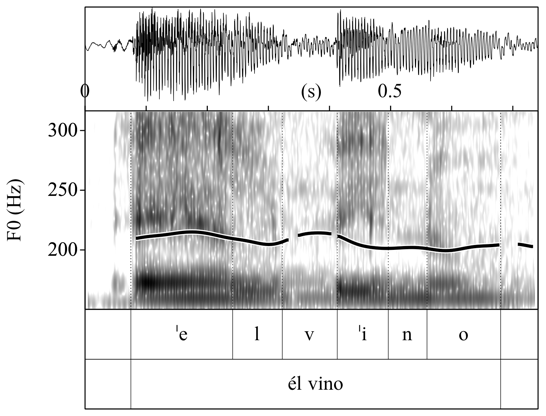
\includegraphics[width=.475\textwidth]{figures/a02HabilTheory-img010.png}\hfill
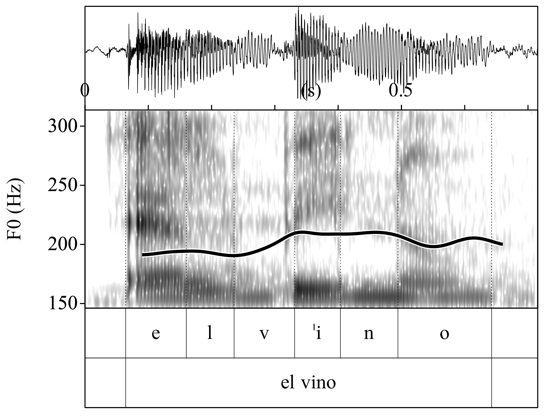
\includegraphics[width=.475\textwidth]{figures/a02HabilTheory-img011.png}
\caption{The pair \textit{él vino} (left) and \textit{el vino} (right) and the influence of orthography on the vowel lengthening in L2 Spanish produced by a L1 Czech learner (F\_07).}
\label{fig:2.9}
\end{figure}


\subsubsection{Syllable structures in contrast}\label{sec:2.3.1.3}

Finally, I will make a brief comment on the combination of segments, that is, on syllable structure. Since German and Czech allow very complex consonant clusters in onsets as well as codas (Czech may even have liquids in the nucleus, e.g., \textit{vlk} ‘wolf’, \textit{prst} ‘finger’), L2 learners have no difficulties with syllable structures in target Spanish and Italian, in which the syllable complexity is much more moderate in terms of the number of possible consonant combinations. Where we might find interferences is in C\#V sequences. In Spanish, the resyllabification rule is systematically applied in connected speech to form “ideal” or prototypical CV syllables (V\textbf{C}\#V → V.\textbf{C}V), as illustrated schematically in \figref{fig:2.10}.



\begin{figure}
%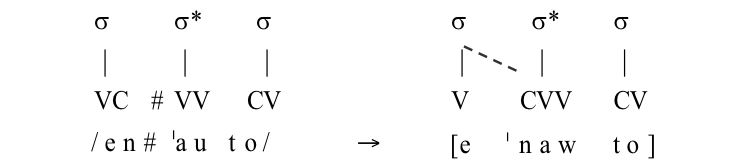
\includegraphics[width=\textwidth]{figures/a02HabilTheory-img012.png}
\begin{forest}
for tree = {align=left,
            baseline=(current bounding box.center)},
[,phantom
  [$\sigma$
    [VC\\/en]
  ]
  [$\sigma$*
    [\#VV\\\#ˈau]
  ]
  [$\sigma$
    [CV\\to/]
  ]
]
\end{forest}
$\to$
\begin{forest}
for tree = {align=left,
            baseline=(current bounding box.center)},
[,phantom
  [$\sigma$, name = s
    [V\\{[e}]
  ]
  [$\sigma$*
    [CVV\\ˈnaw, name = cvv]
  ]
  [$\sigma$
    [CV\\{to]}]
  ]
]
\draw[dashed] (s.south) -- (cvv.north);
\end{forest}
\caption{Example of the CV resyllabification rule that applies in Spanish (\textit{en} \textit{auto} ‘in the car’).}
\label{fig:2.10}
\end{figure}

\begin{sloppypar}
In Italian resyllabification can also occur (\citealt[72]{NesporVogel1986/2007}), whereas German and Czech maintain the word-boundary (\citealt{Szczepaniak2009, ŠimáckováEtAl2012}).\footnote{However, in accordance with phonotactic patterns, resyllabification in Czech is not as strong and prominent as in German. In Moravian Czech, resyllabification is more common than in Bohemian Czech, where the glottal stop is preferred (\citealt[230]{ŠimáckováEtAl2012}).} Such morphological boundaries in vowel-initial words can have different phonetic realizations, comprising mainly glottalization, glottal stop insertion and/or creaky voice (see, e.g., \citealt{ŠimáckováEtAl2012} for Czech; \citealt{Kohler1994,Kohler1995, Pompino-MarschallZygis2010} for German). These strategies can be frequently observed in L2 productions (\figref{fig:2.11}). Spanish and Italian native speakers usually perceive L2 speech without resyllabification and with glottal stops as interrupted and chopped.
\end{sloppypar}



\begin{figure}

%%\includegraphics[width=\textwidth]{figures/a02HabilTheory-img013.tif}
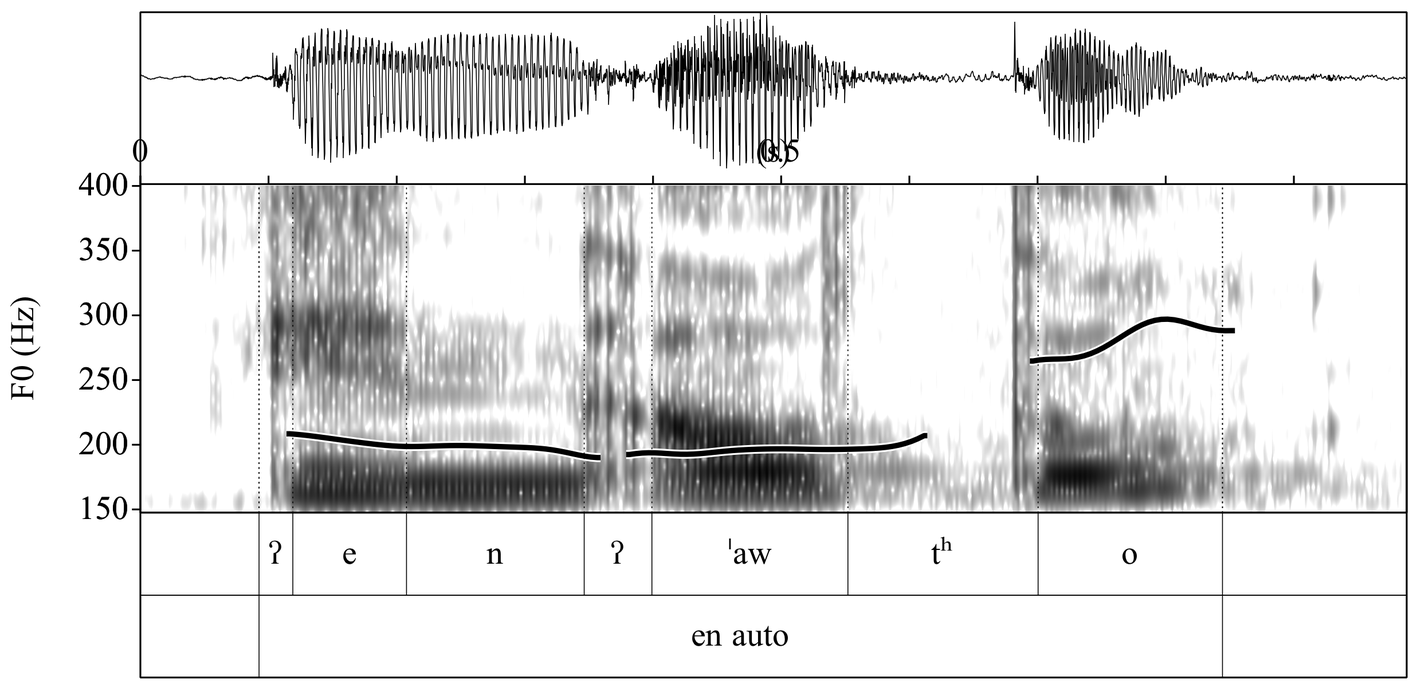
\includegraphics[width=\textwidth]{figures/a02HabilTheory-img013-new.png}



\caption{Insertion of a glottal stop in a C\#V sequence (\textit{en auto}, ‘in the car’) in L2 Spanish produced by an L1 German learner (F\_18).}
\label{fig:2.11}
\end{figure}

Based on this short contrastive analysis and the data gathered in the present study, we can conclude that German learners of Spanish (and potentially of Italian) have more difficulties with the pronunciation of the segments in Romance languages than Czech learners. On the other hand, German shares more prosodic similarities with the Romance languages, as we will see in the next section.

\subsection{Suprasegmental properties in contrast}\label{sec:2.3.2}

As already explained in \sectref{sec:2.2}, intonation serves a variety of linguistic functions such as expressing modality, marking focus and the edges of discourse units, and implementing the lexical accent. In this section, which begins with the presentation of the prosodic typology (\sectref{sec:2.3.2.1}), I will give an overview of other prosodic resources that can also be used to encode these linguistic features and/or are connected directly or indirectly with the use of F0 (\sectref{sec:2.3.2.2}--\sectref{sec:2.3.2.3}). Then, I will present the main tonal patterns of the four languages studied here (\sectref{sec:2.3.2.4}). A summary of their main prosodic features is given in \tabref{tab:2.6a}.

\begin{sidewaystable}
\begin{tabularx}{\textwidth}{QQQQQ}

\lsptoprule

{Prosodic features} & \multicolumn{2}{l}{{Target languages}} & \multicolumn{2}{l}{{L1 backgrounds}}\\
\cmidrule(lr){2-3}\cmidrule(lr){4-5}
& {Italian} & {Spanish} & {Czech} & {German}\\
\midrule
\multirow[t]{2}{=}{Prosodic typology (\citealt{Féry2017, Jun2014})} & {Intonation} language & {Intonation} language & {Phrase} language & {Intonation} language\\
& Head-prominence language & Head-prominence language & Head\slash edge-prominence language & Head-prominence language\\
\tablevspace
Word-stress & Distinctive lexical stress & Distinctive lexical stress & Delimitative stress (fixed on the first syllable) & Distinctive lexical stress\\
\tablevspace
\multirow[t]{2}{=}{Acoustic correlates of stress

(example of pitch track in isolated words)} & Duration, F0, intensity & F0, duration, intensity & No clear correlates & F0, duration, intensity\\
 & 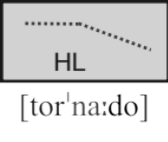
\includegraphics[width=.15\textwidth]{figures/a02HabilTheory-img014.png} & 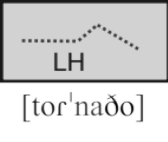
\includegraphics[width=.15\textwidth]{figures/a02HabilTheory-img015.png} & 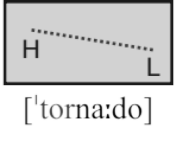
\includegraphics[width=.15\textwidth]{figures/a02HabilTheory-img016.png} & 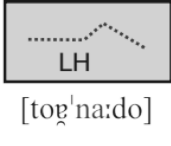
\includegraphics[width=.15\textwidth]{figures/a02HabilTheory-img017.png}\\
\midrule
\end{tabularx}
\caption{Main suprasegmental features of Italian, Spanish, Czech and German in contrast.}
\label{tab:2.6a}
\end{sidewaystable}
\begin{sidewaystable}\ContinuedFloat
\begin{tabularx}{\textwidth}{QQQQQ}

\midrule

{Prosodic features} & \multicolumn{2}{l}{{Target languages}} & \multicolumn{2}{l}{{L1 backgrounds}}\\
\cmidrule(lr){2-3}\cmidrule(lr){4-5}
& {Italian} & {Spanish} & {Czech} & {German}\\
\midrule
Rhythmic isochrony\footnote{The notion of rhythm refers here to the perceptual difference resulting from the isochrony of speech intervals. In very simple terms, syllables in syllable-timed languages tend to have equal duration, whereas intervals between two stressed syllables are equal in stress-timed languages (\citealt{Abercrombie1967} and \citealt{Pike1945}). Spanish and Italian are usually classified syllable-timed languages, whereas German is a stress-timed language (see, e.g., \citealt{Dauer1983, RamusEtAl1999, GrabeLow2002, WhiteMattys2007}), albeit rhythmic characteristics may be less clear cut as shown by, for example, the recent study by \citet{DImperioEtAl2020} for Italian (for criticism or alternative proposals to this traditional isochrony of the rhythm, see, e.g., \citealt{Arvaniti2009}). The rhythm type of Czech has so far not been resolved. \citet{DankovičováDellwo2007} have suggested that Czech is a kind of mixed-stressed language, mainly due to the existence of a contrast between long and short vowels and the syllable complexity that are typical of stress-timed languages.} & Syllable-timed language & Syllable-timed language & {Mixed-timed}

 language & Stress-timed language\\
 \tablevspace
\multirow[t]{2}{=}{Macro-rhythm and tonal density \citep{Jun2014}} & Strong & Strong & Strong(?) & Medium\\
& Dense pitch accent distribution & Dense pitch accent distribution & {Sparer pitch}

 accent distribution & Sparer pitch accent distribution \\
\lspbottomrule
\end{tabularx}


%\caption{Main suprasegmental features of Italian, Spanish, Czech and German in contrast (continued).}
%\label{tab:2.6b}
\end{sidewaystable}

\subsubsection{Prosodic typology and prominence}\label{sec:2.3.2.1}
\begin{sloppypar}
All languages use pitch variation in a meaningful way, but they differ in how pitch is employed for linguistic purposes. Following \citegen{Féry2017} typology, at least four types of languages are distinguished. \textit{Tone languages} (e.g., Chinese Mandarin) make contrastive use of pitch at the lexical level: tones change the meaning of individual words. Tones in \textit{intonation languages} (e.g., English) are specified at higher prosodic levels. As explained in \sectref{sec:2.2}, pitch is used post-lexically for grammatical or pragmatic purposes; in other words, the same sentence can be pronounced with different ``melodies'' according to its function in a discourse. Languages that combine lexical and intonational uses of pitch are called \textit{pitch} \textit{accent languages} (e.g., Swedish). Finally, \textit{phrase languages} (term introduced by \citealt{Féry2010}) share most characteristics with intonation languages, but they also assign phrasal tones (e.g., French).\footnote{Phrasal tones are tones assigned at the level of what \citet{Féry2017} calls a Prosodic phrase (φ phrase), which usually consists of minimally one prosodic word and “that is more or less isomorphic to syntactic phrases, as for instance noun phrases, prepositional phrases or verb phrases” (p. 323). Prosodic phrase is also called Accentual phrase (AP) in the literature (e.g., \citealt{Jun2005, Meisenburg2011}); this term will also be applied in the present study. I will pursue this point later.} This type is very typical for languages with fixed or no lexical stress. Italian, Spanish and German (lexical stress languages) are all prototypical intonation languages, even though they differ from each other, for example, in tonal inventories and in semantic\slash pragmatic meanings of tonal events. As for Czech (a fixed-stress language with initial prominence), it has been proposed that it belongs to phrase languages (\citealt{Pešková2017, PeškováEtAl2018}).
\end{sloppypar}


This typology of language can be further refined according to certain additional criteria. In her model of a prosodic typology, \citet{Jun2005, Jun2014} applies prominence type (head, edge, head/edge) as one parameter for classifying languages.\footnote{This typology of language can be further refined according to certain additional criteria. In her model of a prosodic typology, \citet{Jun2005, Jun2014} applies prominence type (head, edge, head/edge) as one parameter for classifying languages (see \sectref{sec:2.3.2}).} According to this approach, Italian, Spanish and German are \textit{head-prominence languages}, marking phrase-level prominence by the phrase head, which is determined by a metrically strong syllable. This means that a stressed syllable as the head of a word is very important for the anchoring of intonational excursions or pitch accents in all these languages. By contrast, Czech can be seen as a \textit{head/edge-prominence language}, where phrase-level prominence is marked by both, the phrase head and the edge of a phrase. Hence, the main contrast between the two language categories is that a head-prominence language assigns pitch accents associated with stressed syllables, whereas a head/edge-prominence language marks prominence not only with pitch accents but also with boundaries at the phrase level, corresponding to an accentual phrase (AP). Similar to what we see in French, an AP is considered the smallest prosodic phrase (with a break index 2), dominated by an intermediate or intonational phrase. So far there is no broad consensus about the exact characteristics of the AP in Czech, but following \citet{PeškováEtAl2018} and \citet{PeškováForthcoming} we can make at least two main assumptions.\footnote{It can be added that traditional and/or earlier works on Czech intonation (see, e.g., \citealt{Mathesius1937, Ondráčková1954, Palková2017}) call such accentual phrases ``rhythmic'', ``melodic'' or ``speech'' groups/units, which are typical for rhythmic structuring of Czech speech.} First, this small prosodic unit corresponds to at least one lexical word and to all the function words that this lexical word governs (compare with French in \citealt{Delais-RoussarieEtAl2015}). The boundaries of AP generally correspond to syntactic phrases (an in-depth analysis of prosodic phrasing is still required, however). Second, in statements, the stressed syllable is realized mostly with a low pitch level, analysed as L*, and a boundary tone at the edge of the AP with a high peak (Ha) (see an example for Czech in \figref{fig:2.12}). In contrast, the high tones in head-prominence languages such as Spanish or Italian are (mostly) associated with stressed syllables but not the boundary (see an example for Italian in \figref{fig:2.13}).




\begin{figure}
%%\includegraphics[width=\textwidth]{figures/a02HabilTheory-img018.tif}
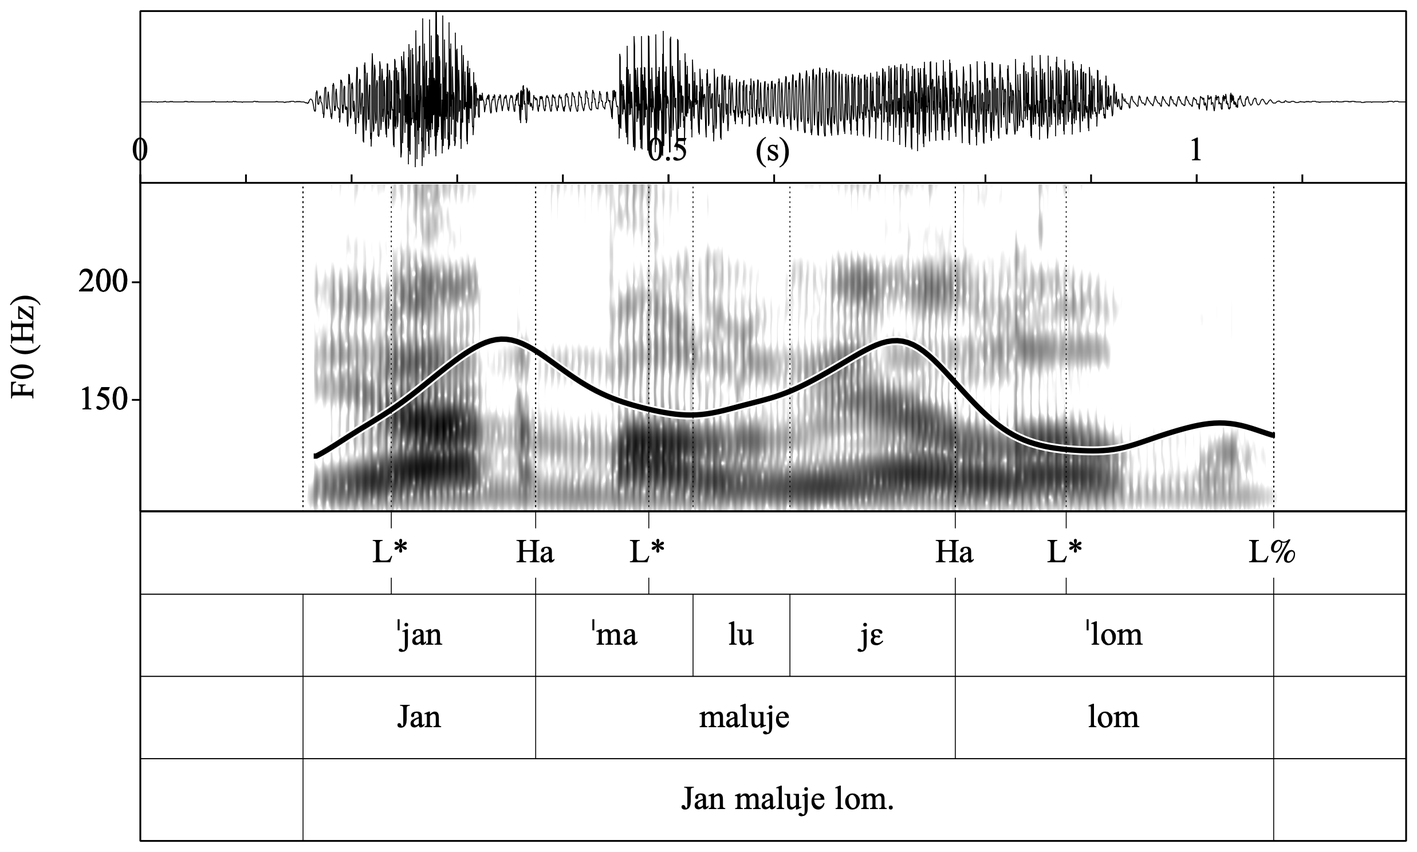
\includegraphics[width=\textwidth]{figures/a02HabilTheory-img018-new.png}



\caption{Waveform, spectrogram, and F0 contour of the broad focus statement \textit{Jan maluje lom} ‘Jan paints a quarry’ in L1 Czech (from \citealt{PeškováForthcoming}).}
\label{fig:2.12}
\end{figure}



\begin{figure}
%%\includegraphics[width=\textwidth]{figures/a02HabilTheory-img019.tif}
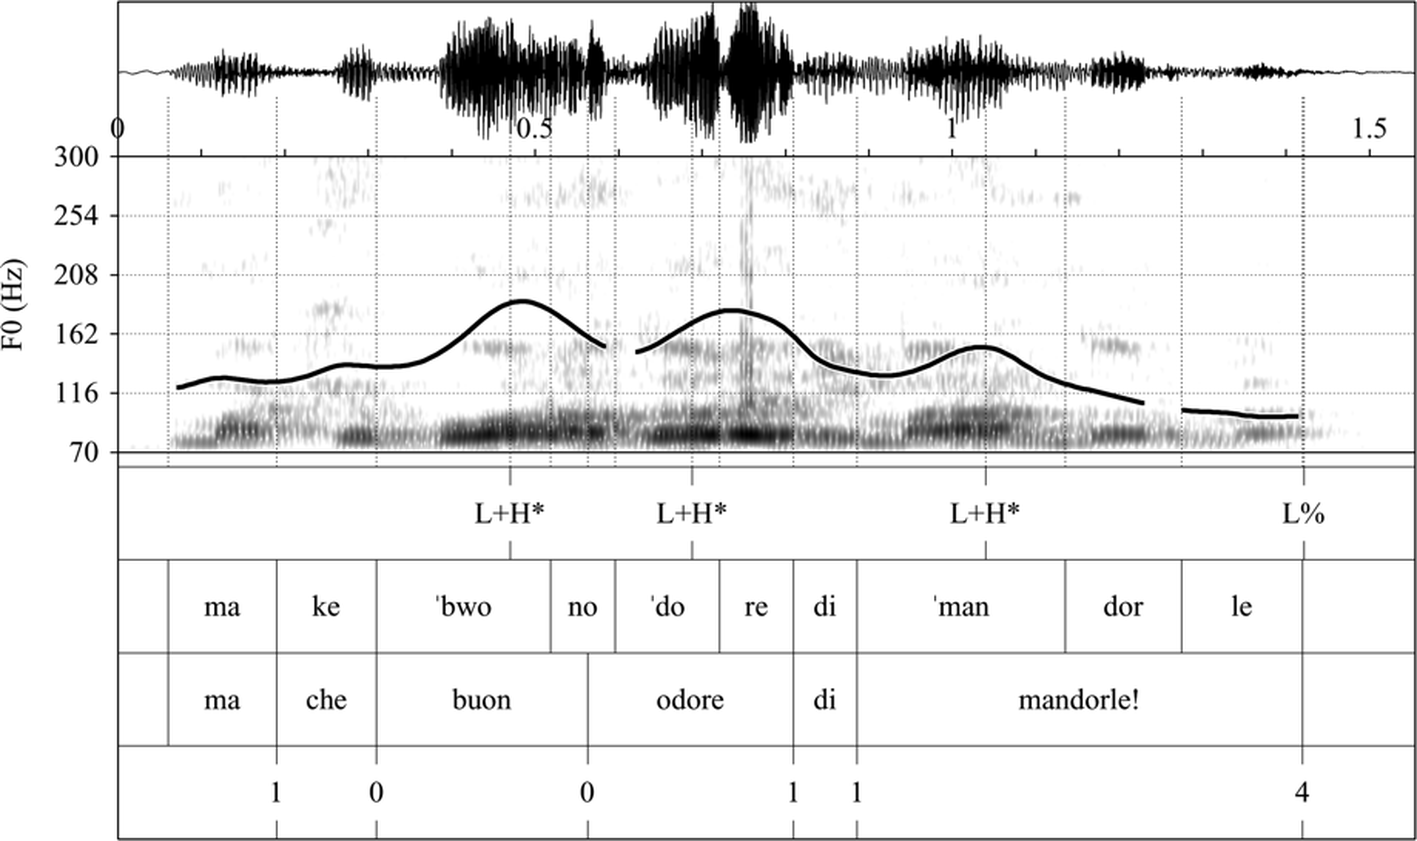
\includegraphics[width=\textwidth]{figures/a02HabilTheory-img019-new.png}



\caption{Waveform, spectrogram, and F0 contour of the exclamative statement \textit{Ma che buon odore di mandorle!} ‘What a good smell of almonds!’ in L1 Italian (from  \citealt[165]{GiliFivelaEtAl2015}, their figure 5.7).}
\label{fig:2.13}
\end{figure}

Interestingly, Czech behaves very similarly to other head/edge-prominence languages such as Bengali (\citealt{HayesLahiri1991, Khan2014}), Tamil \citep{Keane2014} or Hindi \citep{PatilEtAl2008}, which also all have fixed stress on the first syllable. An initial high tone at the very beginning of the utterance is possible, but optional in Czech. Previous work on Czech intonation contemplates additional tonal patterns, including different combinations of L and H tones (see \citealt{Palková1994, Duběda2014}). This variation can be attributed to the number of syllables, expressivity or stylistics, but given the fact that the research on Czech intonation within the AM theory is still in its infancy, further research is still needed in order to fully understand this variation. Considering that the placement of stress plays a role in the prosodic typology introduced above, we will have a closer look at this issue in the following section.

\subsubsection{Lexical stress}\label{sec:2.3.2.2}

All the languages studied here have lexical stress. Stress refers to the degree of relative prominence “that a syllable receives in comparison with the other syllables in a given domain” (\citealt[220]{Hualde2005}, see also  \citealt{GoedemansvanderHulst2013}). Italian, Spanish and German are all lexical stress languages, in which stress has a distinctive function, meaning stress is phonemic and can build minimal pairs (e.g., Sp. [ˈnumeɾo] ‘number’ vs. [numeˈɾo] ‘s/he numbered’). In contrast, Czech is a fixed-stress language, in which stress has a demarcative or delimitative function and is always on the first syllable (e.g., \textit{Praha} [ˈpraha], ‘Prague’). When a monosyllabic preposition precedes a lexical word and both build a single prosodic unit, stress is automatically moved to the very first position (\textit{do Prahy} [ˈdoprahi], ‘to Prague’).


The question is what acoustic correlates are used to convey prominence pattern of the lexical word in the languages under study. German and Spanish use F0 modulation together with duration and/or intensity as important correlates of stress (\citealt{JessenEtAl1995, Jessen1999, Möbius1993} for German;  \citealt{LlisterriBoix1991, LlisterriBoixEtAl2003, Hualde2014} for Spanish). Additionally, German stressed syllables can be identifiable on the basis of the vowel quality too because of vowel reduction in unstressed positions. Whereas F0 appears to be the most significant correlate in Spanish, with duration or intensity as additional strong predictors of stress \citep[245]{Hualde2005}, Italian shows a slightly different picture. The first experimental evidence by \citet{Bertinetto1981} and the results of a recent study by \citet{ErikssonEtAl2016} revealed that duration is the dominant factor of lexical stress in Italian, whereas the role of F0 is secondary. It was also shown that stressed vowels tend to be significantly longer than the corresponding unstressed vowels, regardless of syllable structure. Czech behaves in a very different way from these three languages, exhibiting no clear correlate for stress (\citealt{Volín2010, SkarnitzlEriksson2017}). This might be connected precisely with fixed stress, which is predictable. Interestingly, the posttonic syllable usually receives more prominence -- in the sense of higher values of intensity or a high F0 track. This prominence tends to be sometimes wrongly interpreted as a stressed syllable by foreigners listening to Czech words (\citealt[147]{SkarnitzlEtAl2016}). The first stressed syllable in Czech may also receive such prominence, but this is limited to emphatic or chanted speech and to focus structures (\citealt{SkarnitzlEtAl2016, PeškováForthcoming}, see also \chapref{ch:4}). It could also be suggested that Czech -- similar as, for example, French in some proposals (see, e.g., \citealt{Jun2005, Delais-RoussarieEtAl2015}) -- has not lexical but postlexical stress, meaning that the prominence is assigned to an accentual phrase or other higher prosodic unit. For the time being, I will have to leave this issue unresolved.



Based on the main characteristics of stress, Czech learners usually show more difficulty with the correct placement and/or with the phonetic implementation of stress in Spanish (or Italian) than German learners. An example of this difficulty is given in \figref{fig:2.14} (taken from the data of the reading task carried out for the present study and analysed in \citealt{PeškováEtAl2017}, see \chapref{ch:3}).




\begin{figure}
%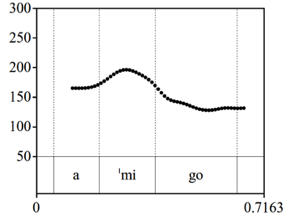
\includegraphics[width=.45\textwidth]{figures/a02HabilTheory-img020.png}
%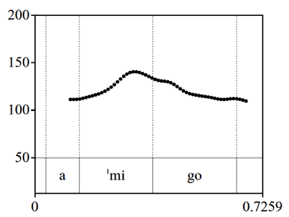
\includegraphics[width=.45\textwidth]{figures/a02HabilTheory-img021.png}




%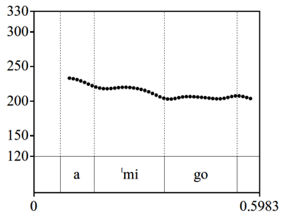
\includegraphics[width=.45\textwidth]{figures/a02HabilTheory-img022.png}
%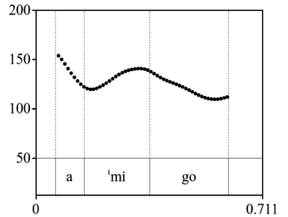
\includegraphics[width=.45\textwidth]{figures/a02HabilTheory-img023.png}
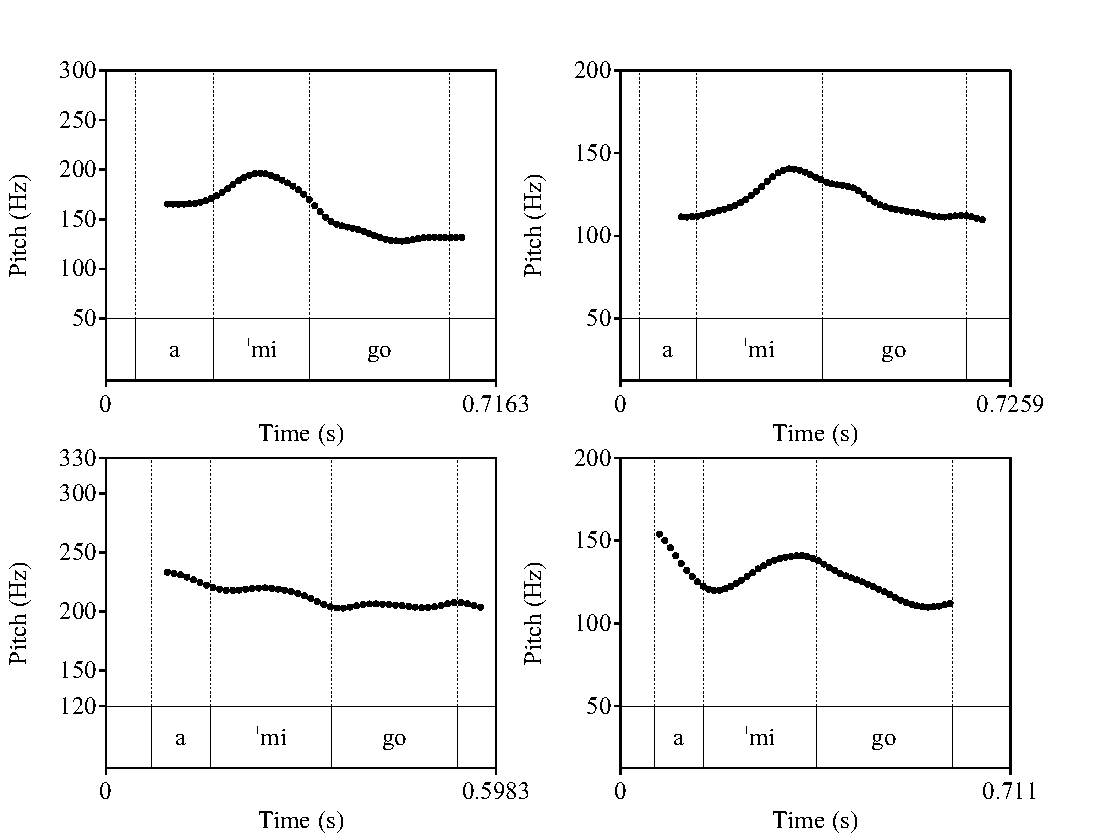
\includegraphics[width=\textwidth]{figures/Figure_2.14.pdf}



\caption{Pitch track of the isolated word \textit{amigo} (‘friend’) in L1 Spanish (at the top left), L2 “German” Spanish (at the top right) and in L2 “Czech” Spanish (below).}
\label{fig:2.14}
\end{figure}

Whereas the German learner of Spanish (\figref{fig:2.14}, picture at the top right) approximates the target pattern (picture at the top left) fairly well, realizing the stressed syllable with a rising F0 movement, the two Czech learners realize it either with a falling pattern from the first syllable or with a target-like pattern and an initial high tone on the first syllable (rightmost picture). Needless to say, such productions were not detected systematically in all Czech learners of Spanish or Italian, but they appeared in the “Czech” L2 data very often and we can therefore call them a typical “Czech” feature. We will see such cases later. Moreover, \citet{PeškováEtAl2017} showed that Czech learners -- especially those at B1/B2 levels -- use durational strategies to express target stress in Spanish, especially when the stressed syllable is not in initial position. Interestingly enough, several Czech words of Spanish origin (see, e.g., \citealt{Ježková2000}) have a long vowel corresponding to the position where the original Spanish word bears stress, as illustrated in \REF{ex:2:1}.


\ea\label{ex:2:1}
\ea \gll {\normalfont Cz.}   \textit{armáda}   {\normalfont /ˈarmaːda/} \normalfont‘army’\\
Sp.   \textit{armada}   /aɾˈmaða/   ‘army’\\


\ex \gll  {\normalfont Cz.}   \textit{kapitán}   \normalfont/ˈkapitaːn/  \normalfont‘captain’\\
Sp.   \textit{capitán}   /kapiˈtan/   ‘captain’\\


\ex  \gll {\normalfont Cz.}   \textit{torpédo}   \normalfont/ˈtorpɛːdo/  \normalfont‘torpedo’\\
Sp.   \textit{torpedo}   /toɾˈpeðo/   ‘torpedo’\\


\ex \gll {\normalfont Cz.}   \textit{generál}   \normalfont/ˈɡɛnɛraːl/   \normalfont‘general’\\
Sp.   \textit{general}   /xeneˈɾal/  ‘general’\\
\z
\z

However, still unanswered are the questions of whether this lengthening is a product of perception or production and why it does not occur with other Spanish borrowings.


The durational effects of stress and syllable complexity together with vowel quantity and quality appear to influence also the speech rhythm of a given language.


\subsubsection{Macro-rhythm and tonal density}\label{sec:2.3.2.3}

Another view on rhythmic properties of languages is proposed by \citet{Jun2014}. She introduces the term \textit{macro-rhythm} and defines it as a tonal rhythm formed within a larger prosodic unit such as an Intonation Phrase. Macro-rhythm together with type of prominence and word prosody represents an important parameter for prosodic typology. Macro-rhythm as a perceived rhythm brought about by changes in F0 differs from \textit{micro-rhythm}, the traditional speech rhythm (see \tabref{tab:2.6a}), which is created by repeated sequences of syllables or feet and which -- according to \citet{Jun2014} -- does not play a role in intonational phonology. \figref{fig:2.15} illustrates the relationship between macro- and micro-rhythm.



\begin{figure}
%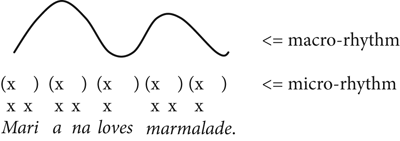
\includegraphics[width=.7\textwidth]{figures/a02HabilTheory-img024.png}
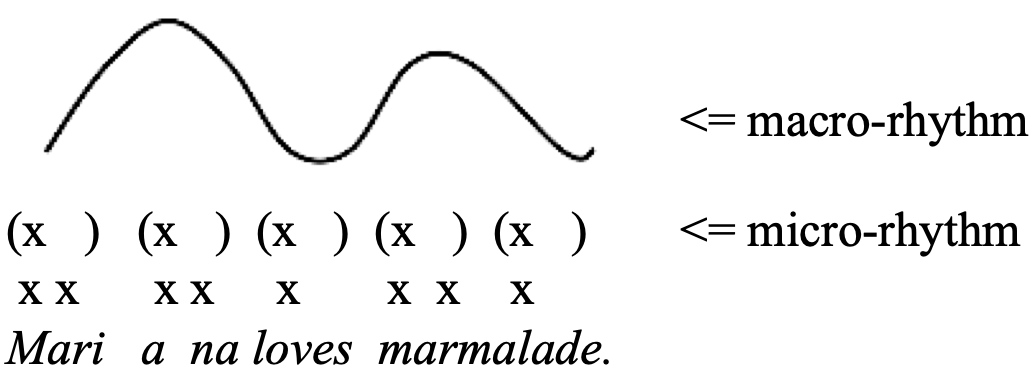
\includegraphics[width=.6\textwidth]{figures/Figure_2.15.png}
\caption{Macro-rhythm and micro-rhythm of the English sentence \textit{Mariana loves marmalade} according to \citet[524]{Jun2014}.}
\label{fig:2.15}
\end{figure}

As explained above, macro-rhythm refers to pitch regularity or repetitions of tonal sequences; fundamental frequency thus contributes to the perception of rhythm in a language and can facilitate word segmentation. Languages differ in the density or sparseness of pitch events in the intonational contour (see also \citealt{Hellmuth2007, FrotaPrieto2015}); in other words, they can exhibit strong, medium or weak macro-rhythm. \citet[525]{Jun2014} proposes three criteria for predicting the degree of macro-rhythm:

\begin{enumerate}[label={(\arabic*)}]\sloppy
\item The \textit{number} of possible phrase-medial pitch accents (PA) or accentual phrases (AP): if a language has fewer alternating types of PA or AP, it is more macro-rhythmic than a language with more variable pitch contours (\figref{fig:2.16}).


\begin{figure}[H]

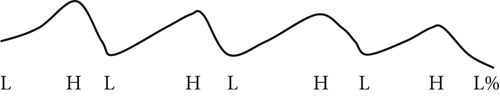
\includegraphics[width=.45\textwidth]{figures/a02HabilTheory-img025.png}

\includegraphics[width=.45\textwidth]{figures/a02HabilTheory-img026.png}


\caption{Stronger macro-rhythm (left) vs. weaker macro-rhythm (right) (from \citealt[525]{Jun2014}).}
\label{fig:2.16}
\end{figure}

\item The \textit{type} of most common PAs or APs: if a language exhibits more rising (LH) or falling (HL) patterns, it is more macro-rhythmic than a language with monotonal levels (H, L) (\figref{fig:2.17}).



\begin{figure}[H]

\includegraphics[width=.45\textwidth]{figures/a02HabilTheory-img027.png}
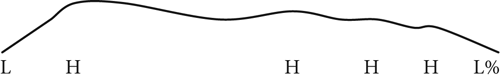
\includegraphics[width=.45\textwidth]{figures/a02HabilTheory-img028.png}




\caption{Stronger macro-rhythm (left) vs. weaker macro-rhythm (right) (from \citealt[525]{Jun2014}).}
\label{fig:2.17}
\end{figure}

\item The \textit{frequency} of PAs and APs: if every word receives PA or AP, then a language is more macro-rhythmic than a language with fewer frequent tonal events (\figref{fig:2.18}).


  \begin{figure}[H]

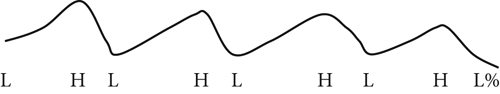
\includegraphics[width=.45\textwidth]{figures/a02HabilTheory-img029.png}
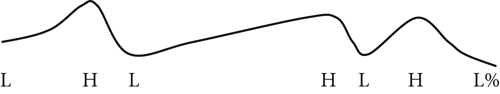
\includegraphics[width=.45\textwidth]{figures/a02HabilTheory-img030.png}




\caption{Stronger macro-rhythm (left) vs. weaker macro-rhythm (right) (from \citealt[525]{Jun2014}).}
\label{fig:2.18}
\end{figure}
\end{enumerate}

According to these criteria, Spanish and Italian are languages with a strong macro-rhythm or a dense pitch accent distribution (\citealt{Jun2014}, see also \citealt{FrotaPrieto2015}), whereas German is a language with a medium macro-rhythm \citep{Jun2014}. Macro-rhythm has not yet been satisfactorily explored for Czech. Nevertheless, the control data collected for this research seem to suggest that Czech also has a strong macro-rhythm (see also \citealt{PeškováForthcoming} for a discussion). Hence, we can conjecture that L2 learners will show more alternations in their production of target pitch accents, precisely because of the differences in the macro-rhythm.


It should be emphasized that \citet{Jun2014} established her typology on the basis of the intonation patterns of declarative sentences described in the literature. And as she notes (\citeyear[539]{Jun2014}), “the degree of macro-rhythm could change if we add other sentence types or include speech materials produced in different styles of speech.” Here further research is needed to quantify macro-rhythm across various languages and data.


\subsubsection{Tonal inventories in contrast}\label{sec:2.3.2.4}

The comparison of intonation patterns serves as a point of departure for the examination of L2 pitch contours in the present study; these are extensively treated in \chapref{ch:4}. Before I start presenting a summary of the main tonal patterns of the languages under study and offering an overview of AM labels used for the annotation of intonational contours, the previous research on intonation is briefly summarized in \tabref{tab:2.7}. Unfortunately, not all work done in this area can be listed here. I have therefore selected only some of them, which also offer important overviews and references for further reading. In general, the research on the intonation of each language under study has a very long tradition, dating back at least to the first half of the 20th century. The earliest of these intonational studies were mostly of a purely descriptive nature based on auditory analysis, but they provide very valuable information on how the ``melody'' of these languages works and sounds like. With the publication of \citegen{Pierrehumbert1980} thesis, interest in intonational phonology spread rapidly and since then the number of studies within the AM framework has greatly increased (some other approaches were mentioned in \sectref{sec:2.2}). It must be noted here that in comparison to Spanish, Italian and German, the modelling of Czech intonation within the AM framework, which started with \citet{Duběda2011, Duběda2014}, is still very limited.

\vfill
\begin{table}[H]
\begin{tabularx}{\textwidth}{lQQQQ}
\lsptoprule
 & \multicolumn{2}{c}{{Target languages}} & \multicolumn{2}{c}{{L1 backgrounds}}\\\cmidrule(lr){2-3}\cmidrule(lr){4-5}
Approach & { Italian} & { Spanish} & { Czech} & { German}\\
\midrule
Non-AM &  \citealt{AgardDiPietro1965, Fiorelli1965, LepschyLepschy1977, DEugenio1982, Canepari1985} &  \citealt{NavarroTomás1948, Quilis1975,Quilis1987} & \citealt{Chlumský1928, Petřík1935a, Petřík1935b, Mathesius1937, Daneš1957,Daneš1985, Grepl1965, Romportl1972, Palková1994,Palková2017} & \citealt{Klinghardt1923, vonEssen1964, Pheby1975, Kohler1991a, Kohler1991b, Fox1984, Selting1995, Peters1999}\\\tablevspace
AM & \citealt{Avesani1990, Grice1995, Rabanus2001, DImperio2002, GriceEtAl2005b, Cangemi2014, GiliFivelaEtAl2015} & \citealt{Sosa1999, Hualde2003, Face2002, FacePrieto2007, BeckmanEtAl2002, AguilarEtAl2009, PrietoRoseano2010, HualdePrieto2015} & \citealt{Duběda2011, Duběda2014, Pešková2017, PeškováEtAl2018, PeškováForthcoming} & \citealt{Féry1993, Grabe1998, Wunderlich1988, Uhmann1991, GriceBaumann2002, GriceEtAl2005a}\\
\lspbottomrule
\end{tabularx}

\caption{Selected works on the intonation of Italian, Spanish, Czech and German.}
\label{tab:2.7}
\end{table}
\vfill\pagebreak

Since the present study was carried out within the AM framework, work undertaken within this approach has been consulted in order to provide the descriptions of tonal sequences. Although we have gained a lot of knowledge about intonation in these languages, research still shows certain limitations (some of the weak points were already discussed in the previous section). First, the proposed (phonological) inventories of tonal patterns (see below) are usually built upon just a few speakers, considering inter-speaker variation to a limited extent (if at all). Second, many studies focus predominantly on the realization of nuclear pitch accents and boundary tones rather than on prenuclear positions, and the “non-phonological” parts between two tonal events are mostly ignored altogether. The reason for not including these parts in the analysis is that they do not convey meaning or do not establish contrasts and are thus less interesting for phonology, in comparison with the nuclear configurations. Though this is certainly true, languages can still differ considerably here and thus “sound” differently. Third, we still lack a comprehensive and “universal” application for the analysis of a large number of (not only dialectal) varieties (the question of regional variation will be addressed below). And, finally, the relationship between F0 and different meanings is still a hot topic too, partly due to the fact that other prosodic cues (intensity, duration etc.) may interact strongly with F0 (see, e.g., \citealt{NiebuhrWinkler2017}).


In spite of these limitations, substantial work has already been done, and the suggested inventories based on acoustic performance allow us to understand the composition of intonation and to compare different tonal patterns within as well as across languages. According to the literature and the intonational analyses contained therein, the tonal inventories of the languages studied here are made up of monotonal and bitonal pitch accents and monotonal and bitonal boundary tones. Tritonal accents represent exceptions. Additionally, Czech as a head/edge-prominence language assigns two types of boundary tones of AP too (Ha, La).\largerpage



\tabref{tab:2.8a} offers an overview of tonal inventories assumed for the languages under study based on previous research. Though the languages have a great deal in common, they differ from each other in how they assign tonal events and in the meanings they convey with these sequences. I will present details in \chapref{ch:4}. At first glance we can see that Spanish and Italian are intonationally “richer” languages in comparison to Czech and German. This concerns in particular the possible combination of pitch accents and boundary tones, called nuclear configurations (NC). (The “rich” inventory of NC in Italian is also due to the range of dialects included here.) As we will see, one nuclear configuration can convey more meanings in every language. For example, in Spanish and Czech, a L* L\% nuclear configuration is found in both (neutral) declaratives as well as in wh-questions (\citealt{Estebas-VilaplanaPrieto2010, Pešková2017}). In Italian, H+L* L\% has a broad range of meanings, including broad-focus as well as narrow-focus statements, exclamatives, wh-questions, or imperative requests (\citealt{GiliFivelaEtAl2015}). And, finally in German, H* L-\% is described for neutral statements and wh-questions (\citealt{GriceBaumann2002}).


\begin{table}[p]
\small
\begin{tabularx}{\textwidth}{QQQQQ}

\lsptoprule

Intonation  & \multicolumn{2}{l}{{Target languages}} & \multicolumn{2}{l}{{L1 backgrounds}}\\
\cmidrule(lr){2-3}\cmidrule(lr){4-5}
inventory\footnote{Sp\_ToBI (\textit{Training materials}) can be found at the following link: \url{http://prosodia.upf.edu/sp\_tobi/en/} (22.6.2019) (cf. \citealt{AguilarEtAl2009}). GToBI (\textit{Übungsmaterialien zur deutschen Intonation}) can be found at the following link: \url{http://www.gtobi.uni-koeln.de/index.html} (22.6.2019) (cf. \citealt{GriceBaumann2002}).} & {Italian}

 (\citealt{GiliFivelaEtAl2015}) & {Spanish}

 (Sp\_ToBI) & {Czech}

 (Cz\_ToBI: work in progress) & {German}

 (G\_ToBI)\\
 \midrule
{Pitch accents} & { L*}

{ H*}

{ H+L*}

{ L+H*}

{ L+<H*}

{ L*+H}

{ L*+>H}

{ H*+L}

{ L+¡H*} & { L*}

{ H*}

{ H+L*}

{ L+H*}

{ L+<H*}

 L*+H & { L*}

{ H*}

{ (H+L*)}

{  (L+H*)\footnote{The phonological status of the L+H* and H+L* in Czech remains unresolved and is discussed in \citet{PeškováForthcoming}.}}

{ L*+H} & { L*}

{ H*}

{ H+L*}

{ L+H*}

{ L*+H}

 H+!H*\\
 \tablevspace
{Boundary tones (AP)} & -- & -- & Ha, La & --\\
\tablevspace
{Boundary tones (ip, IP)} & {L\%}

{ H\%}

{ H!H\%}

{ LH\%}

{ L!H\%}

 HL\% & { L\%}

{ H\%}

{ !H\%}

{ LH\%}

{ L!H\%}

{ HL\%}

 LHL\% & { L\%}

{ H\%}

{ (H)!H\%}

{ LH\%}

{ Hː\%}

 Lː\% & { L\%}

{ H\%}

{ !H\%}

{ LH\%}

 H-\^{}H\%\\
 \midrule
 \end{tabularx}
 \caption{Comparison table for the tonal inventories of Italian, Spanish, Czech and German. The diacritics have the following meaning: \textit{>H*}  indicates H earlier alignment (vs. \textit{<H*} a later alignment), and \textit{\^{}} is another symbol for an upstep.}
 \label{tab:2.8a}
 \end{table}
 
 \begin{table}[p]\ContinuedFloat
 \small
 \begin{tabularx}{\textwidth}{p{.22\textwidth}QQQQ}

 \midrule

 Intonation  & \multicolumn{2}{l}{{Target languages}} & \multicolumn{2}{l}{{L1 backgrounds}}\\
 \cmidrule(lr){2-3}\cmidrule(lr){4-5}
 inventory & {Italian}

  (\citealt{GiliFivelaEtAl2015}) & {Spanish}

  (Sp\_ToBI) & {Czech}

  (Cz\_ToBI: work in progress) & {German}

  (G\_ToBI)\\
  \midrule
{Nuclear

configurations} & { H* L\%}

{ H* LH\%}

{ H*+L L\%}

{ H*+L LH\%}

{ H+L* HL\%}

{ H+L* L\%}

{ H+L* LH\%}

{ L*+>H L\%}

{ L*+H H\%}

{ L*+H HL\%}

{ L*+H L\%}

{ L+¡H* H\%}

{ L+¡H* L\%}

{ L+¡H* LH\%}

{ L+H* H!H\%}

{ L+H* H\%}

{ L+H* L!H\%}

{ L+H* L\%}

{ L+H* LH\%}

 L+H*(+L) L\%\footnote{As stated in  \citet[192]{GiliFivelaEtAl2015}, there are two different realizations of /L+H* L\%/ in Italian, depending on whether the high tone is aligned with the end or with the middle of the stressed syllable. I have used the label L+H*(+L) for the latter case in order to mark this difference. This pattern has been observed in different Italian varieties and in different contexts such as contrastive-corrective narrow-focus statements.} & { H* !H\%}

{ H* HL\%}

{ H* L\%}

{ H+L* HH\%}

{ H+L* HL\%}

{ H+L* L\%}

{ H+L* LH\%}

{ L* HH\%}

{ L* HL\%}

{ L* L!H\%}

{ L* L\%}

{ L* LH\%}

{ L+¡H* L\%}

{ L+H* !H\%}

{ L+H* HH\%}

{ L+H* HL\%}

{ L+H* L\%}

{ L+H* LH\%}

 L+H* LHL\% & { L* (H*) L\%}

{ L*+H (L+H*) L\%}

{ L* (L)H\%}

{ L*+H !H\%}

{ L*+H H\%}

{ L*+H LH\%}

{ L*+H !Hː\%\footnote{In \citet{PeškováEtAl2017}, I argue that the final lengthening (H:\%, L:\%) is phonological in (familiar) exhortative and insistent requests.}}

{ L*+H Lː\%}  & { H* L-\%}

{ H+!H* L-\%}

{ H+L* L-\%}

{ L* H-\^{}H\%}

{ L* L-H\%}

{ L*+H L-\%}

{ L+H* !H\%}

{ L+H* H-\%}

{ L+H* H-\^{}H\%}

{ L+H* L-\%}

 L+H* L-H\%\\
\lspbottomrule
\end{tabularx}
\caption{Comparison table for the tonal inventories of Italian, Spanish, Czech and German (\textit{continued}).\label{tab:2.8b}}
\end{table}

One issue related to the intonation patterns presented should be raised here. The Spanish ToBI is based on Peninsular Spanish, German ToBI on the Northern German spoken variety and Czech ToBI on Moravian and Bohemian dialects, whereas the Italian ToBI illustrates contours of different regional varieties across Italy. Since we know that dialects differ in terms of prosody, the question is how to treat this variation in SLA and L2 classes. In comparison to the acquisition of non-native segments, which can be more easily oriented to the “ideal” (albeit sometimes artificial) native model, the intonation represents a phenomenon that is relatively difficult to “standardize”. Another challenging issue related to the present study was to find participants who had been exposed to a single L2 variety and yet fulfilled also other criteria. This is especially the case of students who have studied an L2 in a classroom in their home country, as is the case of the present study. I will return to this issue in more detail in Chapters~\ref{ch:3}, \ref{ch:4} and~\ref{ch:5}.


Coming back to the tonal patterns presented in \tabref{tab:2.8a}, it must also be added that the tonal inventory for Czech proposed here is preliminary because work on Czech intonation within AM is still in progress. The present proposal does not differ from the Czech intonational grammar suggested in \citeauthor{Duběda2011}’s earlier studies (\citeyear{Duběda2011, Duběda2014}), the only difference consisting of the fact that I treat Czech as a phrase language and assume phonological APs. We also observe that this language exhibits the most limited tonal inventory. On the other hand, it shows a larger phonetic “flexibility” within the AP domain. For instance, the underlying tone /L*+H/ appears to be implemented phonetically as L+H* (or L+<H*), which is subject to the length of a word. Whether there might be a phonological difference between L+H* and L*+H in some instances is not clear so far. Nor is it clear whether H+L* should be included in the tonal inventory. \citet[88]{Duběda2014} incorporates this prenuclear “accentual peak”, consisting of a falling contour between the stressed and the posttonic syllable, into his inventory. In my approach, such falling patterns can be seen as a mere phonetic implementation of L* within a default AP (L* Ha). Furthermore, Czech pitch contours share a lot of phonetic similarities with the other three intonation languages, but for phonological reasons, the same F0 movement is labelled differently. An example is given in Figures \ref{fig:2.19} and \ref{fig:2.20}. Here the nouns \textit{pomeranče} (Czech) and \textit{naranjas} (Spanish) (‘oranges’), which both are in focus, are analysed differently: L*+H (i.e., low tone on the accented syllable and rise on the posttonic syllable) in Czech vs. L+H* (i.e., rising tone on the accented syllable and fall on the posttonic syllable) in Spanish, respectively. But note that the pitch movement of the focus domain is almost the same in that we have here one word with more than two syllables realized with a low pattern on the first syllable (the stressed one in Czech), followed by a sharp rise on the second syllable (the stressed one in Spanish); the last syllable(s) is/are realized with a fall and low tone.\footnote{Notice that the final AP in an ip or an IP does not bear phrasal tones (La, Ha) due to the so called \textit{concurrent boundary tone overriding} (term used in \citealt{Khan2014} for Bengali). This is valid for final accentual phrases.}




\begin{figure}[p]
%%\includegraphics[width=\textwidth]{figures/a02HabilTheory-img031.tif}
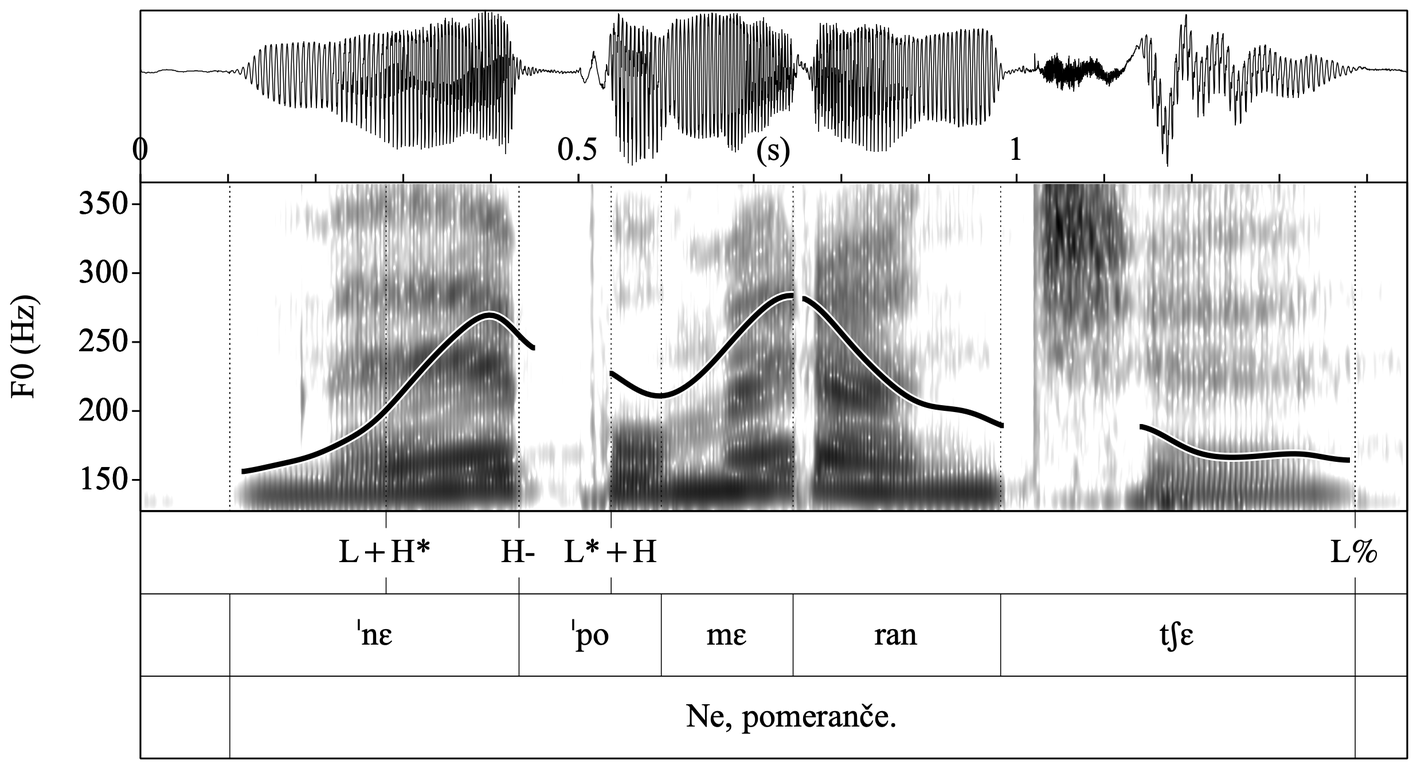
\includegraphics[width=\textwidth]{figures/a02HabilTheory-img031-new.png}
\caption{Focus marking in a narrow focus statement \textit{Ne, pomeranče!} (‘No, oranges!) in L1 Czech.}
\label{fig:2.19}
\end{figure}


\begin{figure}[p]
%%\includegraphics[width=\textwidth]{figures/a02HabilTheory-img032.tif}
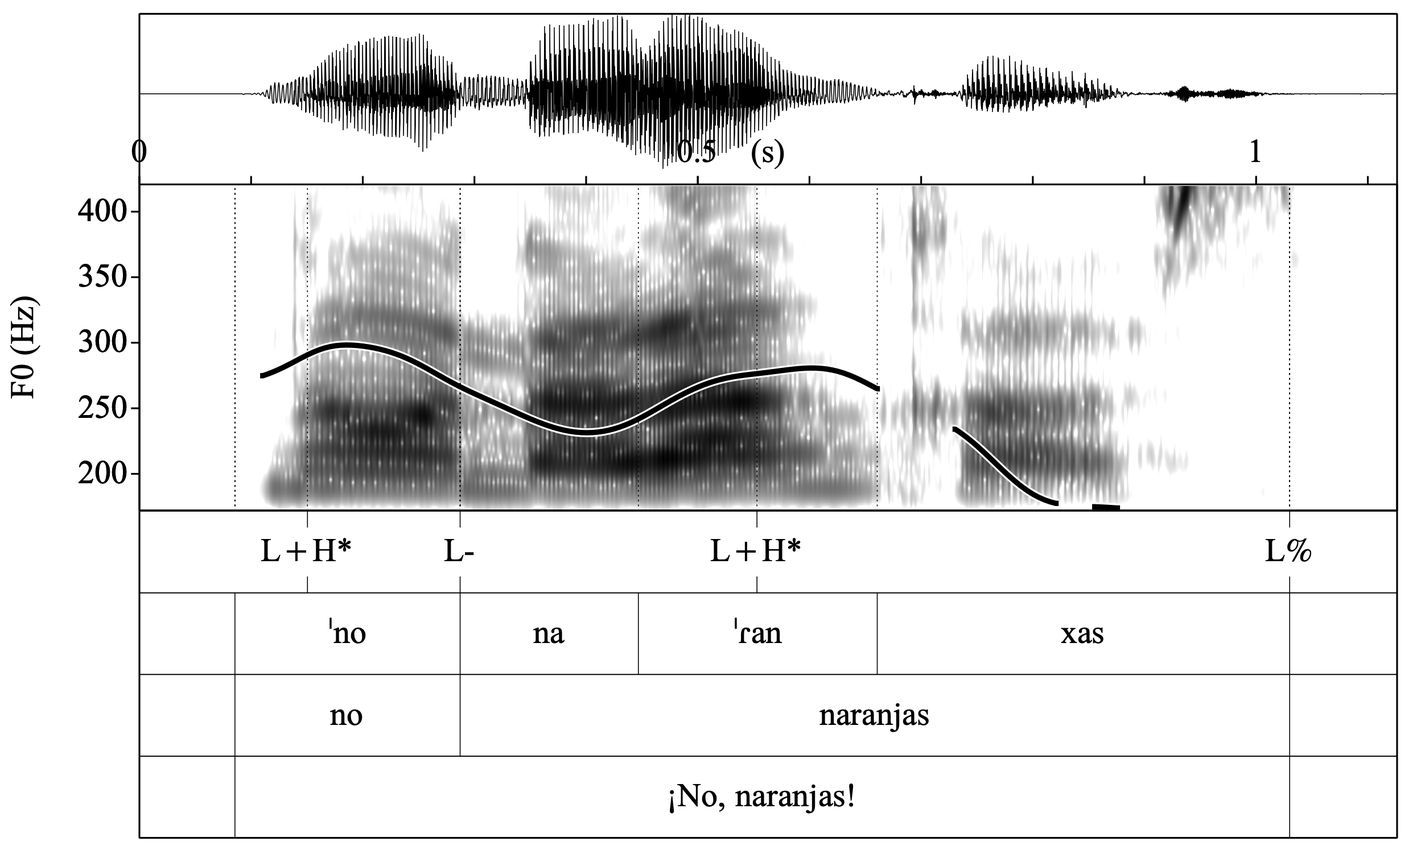
\includegraphics[width=\textwidth]{figures/a02HabilTheory-img032-new.png}

\caption{Focus marking in a narrow focus statement \textit{¡No, naranjas!} (‘No, oranges!) in L1 Spanish.}
\label{fig:2.20}
\end{figure}

In sum, all languages can display contours that are phonetically the same but phonologically different; and the other way round, they can have contours that may be phonologically the same but phonetically different.


With reference to the tonal inventories presented above and findings reported in the previous research, we can expect CLI in L2 productions. The central question is which (if any) tonal targets are produced in a target-like manner and which features from L1 are transferred in L2 and why. These issues are considered properly in the fourth chapter, which describes intonation patterns according to four -- both neutral and non-neutral -- sentence types (declaratives, yes/no questions, wh-questions and vocatives) and formulates hypotheses based on similarities and dissimilarities seen across the languages under study. Before coming to the results regarding intonation patterns in L2 Italian and L2 Spanish in \chapref{ch:4}, in the section that follows I present various theoretical approaches and proposals related to modelling of L2 speech and L2 intonation.


\section{Models of L2 speech acquisition}\label{sec:2.4}
\largerpage
Up to now, it was explained what L2 speech means and which goals research on L2 speech pursues, what factors may shape a foreign accent and explain individual learner differences (\sectref{sec:2.1}), how intonation is defined and modelled (\sectref{sec:2.2}), and, finally, in which ways the languages under study differ in terms of segmental and suprasegmental phonology (\sectref{sec:2.3}). This section presents and discusses various theories and models that have attempted to interpret CLI and to predict what kinds of difficulties or errors occur in non-native speech. Many theoretical proposals have been put forth, both production-based and perception-based, and it will not be possible to cover all of them here. Rather, this attempt to come to a closer understanding of the processes in L2 acquisition will be grounded in a limited selection of approaches (for overviews as well as discussions of the different theoretical approaches, see, e.g., \citealt{Eckman2004, ColantoniEtAl2015, DerwingMunro2015}). Since the present study deals with L2 intonation, I find of particular interest \citegen{Mennen2015} \textit{L2 Intonation Learning theory}, which is based on the AM framework fundamental to the present study. Before introducing the LILt in \sectref{sec:2.4.2}, I will establish a foundation with contrastive analysis.


\subsection{Contrastive analysis}\label{sec:2.4.1} %2.4.1 /
\largerpage
It could be said that modern research on the role of cross-linguistic influences started with two seminals books, \citegen{Weinreich1953} \textit{Languages in Contact} and \citegen{Lado1957} \textit{Linguistics Across Cultures.} Whereas the first of these texts made an important contribution to the role of L1 in L2 in research on contact linguistics and linguistic change, the second laid the groundwork for the theoretical contrastive study of languages with important implications for teaching. Lado’s \textit{Contrastive Analysis Hypothesis} (CAH) suggests working procedures to carry out the systematic comparison of the L1 and L2, including sound systems, grammatical structures, vocabularies, on one hand, and writing systems and cultures, on the other. The systematic comparison of the two languages makes it possible to predict learning difficulties and to show where improvement is needed. One of the central assumptions of the CAH is that learners will have much more difficulty producing and perceiving anything that is “new”. Taking an example from a comparison of sound systems, Lado says that learners will have more problems distinguishing and reproducing sounds that do not exist in their L1s than with sounds that are already present in their L1s.\footnote{\citet[51--52]{Trubetzkoy1969} in his \textit{Principles of Phonology} describes the process of L2 learning in a similar way; he calls it “false evaluation of the phonemes of a foreign language.” According to him, “[e]ach person acquires the system of his mother tongue. But when he hears another language spoken he intuitively uses the familiar ‘phonological sieve’ of his mother tongue to analyse what has been said. However, since this sieve is not suited for the foreign language, numerous mistakes and misinterpretations are the result. The sounds of the foreign language receive an incorrect phonological interpretation since they are strained through the ‘phonological sieve’ of one’s own mother tongue.”} This generalization provoked broad debate and was repeatedly refuted by posterior studies offering evidence that new sounds do not always present difficulties for L2 learners (see, e.g., \citealt{Flege1987, Flege1995, Brown1998}). As for prosody, Lado formulates the following difficulty with regard to the learning of L2 intonation: when the L1 has many levels of pitch (Lado calls them \textit{pitch phonemes}), it is easier to learn a language that contains fewer. With regard to intonation patterns (a set of pitch phonemes within a phrase) in particular, he concludes: “Most of the intonation problems stem from patterns which are the same in form in the two languages but have a different meaning in each” \citep[44]{Lado1957}. This is what \citet{Ladd1996, Ladd2008} and \citet{Mennen2015} call the \textit{semantic} \textit{dimension} (I will come to this issue later). Lado’s generalization holds especially true for a comparison of two intonation languages. According to him, native speakers of tonal languages will have greater difficulty learning intonation languages than tonal languages, just as will native speakers of intonation languages learning a tonal language. Here too, however, research suggests that this need not always be the case. For example, the study on L2 English intonation by \citet{Ortega-LlebariaColantoni2014} showed that Spanish learners transferred more L1 patterns and produced somewhat “worse” English focus marking than (Mandarin) Chinese learners did. The CAH thus seems to be untenable in certain respects. \citet[64--65]{DerwingMunro2015} summarize the weaknesses of the CAH in four points: (1) the CAH does not treat perception and production separately, (2) it does not account for changes in interlanguage over time, (3) it does not explain individual learner differences and (4) it does not clarify the underlying cognitive processes that lead to pronunciation errors. Posterior models and theories have focused especially on the interrelation between production and perception, since perception has been shown to be crucial for both L1 and L2 acquisition of sound systems in general. Moreover, it has been proved that L2 learners also have “perceptual foreign accents”, meaning that learners perceive TL sounds differently than natives of this language do (\citealt[22]{Strange1995}, see also \citealt{McAllister1997}). Nonetheless, in spite of the CAH’s weaknesses, contrastive (and comparative) analysis \textit{per se} still plays a crucial role in different areas of theoretical as well as applied linguistics. After all, it appears to be what (especially adult) learners tend to do as soon as they start to learn a new language: they compare it with their L1 and notice divergent features -- at least the most marked ones. To date, various approaches, both theoretical and empirical, that involve contrastive, error or interlanguage analysis have been set out. Of particular note within second language learning is the method called \textit{Contrastive Interlanguage Analysis} (CIA), introduced in 1996 by Granger for purposes of learner corpus research with a main focus on English as L2 (for a revision of the model, see also \citealt{Granger2015}). As already mentioned in the \textit{Introduction}, I chose this design method because it combines a comparison of non-native and native speakers of a language, on one hand, and a comparison of non-native speakers of a language with different L1 backgrounds on the other. What is new in my study is an additional scenario: a comparison of non-native speakers with the same L1 background who are learning different TLs.



Since the main focus of the present research is on the production of intonation patterns, I will follow \citegen{Mennen2015} \textit{L2 Intonation Learning theory} (LILt), which considers several generalizations from perception- and production-based theories in order to explain the principles which govern the acquisition mechanisms of intonation.


\subsection{L2 Intonation Learning theory \citep{Mennen2015}}\label{sec:2.4.2}

The main motivation behind this theory, which is based on the AM model, is twofold, namely that L2 learners exhibit CLI in L2 intonation, even at a very advanced level, and that research and models of L2 speech have limited utility for the production and perception of segmental phenomena. The LILt provides first a cross-language comparison that allows the identification of L2 intonation “errors” (see \sectref{sec:2.4.2.1}) and then general theoretical assumptions which incorporate different models of L2 (segmental) speech and adjust them to the acquisition of L2 intonation (see \sectref{sec:2.4.2.2}).


\subsubsection{Cross-language comparison and the identification of L2 intonation deviations}\label{sec:2.4.2.1}

Cross-language (and cross-varietal) comparison is the first step assumed in the use of the LILt method. The researcher must describe the L1 intonation patterns and then compare them with L2 intonation patterns, taking into account four central dimensions of cross-linguistic variation, namely the (1) systemic, (2) phonetic, (3) semantic and (4) frequency dimensions (cf. \citealt{Ladd1996,Ladd2008}). Once this comparison is carried out it is then possible to predict where L2 intonation deviations are likely to occur and identify them accurately.



Regarding the first -- systemic -- dimension (inventory and distribution of categorical phonological elements), Spanish and Italian have rich intonation systems and exhibit more different types of pitch accents and boundary tones than German and Czech (see \tabref{tab:2.8a} in \sectref{sec:2.3.2.4}). For example, Spanish LHL\% boundary tones or Italian H*+L and L*+>H pitch accents do not appear in Czech and German at all. The languages also permit different combinations of tonal events. There are clearly more nuclear configurations in the two Romance languages, meaning that these languages use more tones to convey different meanings (we will come to the semantic dimension below). By contrast, Czech and German may either be intonationally ambiguous or compensate for “missing” patterns with other prosodic or syntactic strategies or the use of lexical items such as particles or adverbs. It should be added that Czech also uses further devices for the expression of biased sentences instead of intonation or lexical items, such as different ways of articulation of the segments or changes in F0 span and level (the latter strategies are based on my impressionistic observation and native intuition and deserve systematic investigation in future). It should be added that across and within languages, some sentence types (e.g., narrow focus statements) show tonal consistency, whereas other sentence types (e.g., yes/no questions) display high variation. The four languages under study here differ in their tonal inventories (see, e.g., \citealt{FrotaPrieto2015} for various Romance languages) and we will deal with this and other dimensions properly in \chapref{ch:4}, when results on L2 Spanish and L2 Italian intonation patterns will be reported. At least two questions related to this dimension arise: \textit{Will L2 learners omit those pitch accents and boundary tones that do not form part of their native language inventory? Will they transfer their native patterns that are not present in the target language}? For example, \citet{Mennen2015} reports that neither Italian nor Punjabi learners of the same variety of English produce complex pitch accents H*LH and L*HL, which are present in the L2 in question but absent in their respective L1s.\largerpage



With regard to the second (phonetic or realisational) dimension, the four languages also differ in how tonal tunes are phonetically implemented. Most importantly, this dimension refers to the realization of the tonal alignment, tonal scale and tonal slope. For example, Spanish shows a high sharp final rise in yes/no questions, which reaches a very high frequency in the speaker’s range, in comparison to Czech or Italian. Originally, Sp\_ToBI proposed the label HH\% for this type of a very high rising movement, which was later changed to a “simple” monotonal H\% (\citealt{PrietoRoseano2010}). Another example is the realization of rising accents in prenuclear positions of broad focus statements (and further possible types of utterances too). Italian and German exhibit mostly an earlier peak alignment within the stressed syllable, whereas Spanish has delayed peaks. In Czech, a phrase language, the situation is slightly different. For example, when the AP is mono- or disyllabic, it has an earlier alignment (within the stressed syllable), and when it has three or more syllables, the rise is aligned with the posttonic syllable or later. So here the question is: \textit{Will learners have particular problems with realization of target-like scaling or alignment of pitch contours?}\footnote{My study will focus especially on alignment and on pitch change. Measurements of slope properties and other phenomena are left for the future.} For example, \citet{Mennen2004} showed by means of a reading task of declarative sentences that a majority of the Dutch learners of Greek she examined (who all had 12–35 years of experience with the TL) tended to align the prenuclear peak much earlier than native Greek speakers. This finding on deviations in pitch alignment supported evidence elsewhere on the influence on L2 intonation of an L1. \citet{TrofimovichBaker2006} reported similar tendencies in the production of English by Korean adult learners, but revealed that the “erroneous” peak alignment did not contribute to the perception of a foreign accent. Interestingly, peak alignment also played no role in foreign accent in Korean children learners of English in a posterior study by \citet{TrofimovichBaker2007}. In contrast, stress timing, speech rate, pause frequency and pause duration showed effects in accentedness ratings in both studies.



Furthermore, the four languages show significant contrasts in the semantic dimension or functionality of the tunes, meaning that their tonal distribution is not the same. For example, L*+H has been described for the focus domain in Czech, but in Spanish for prenuclear accents of yes/no questions. Wh-questions in Spanish have predominantly falling patterns, but in German they commonly end in rises, depending on their pragmatic status. (Neutral) vocatives in German, Spanish and Italian mostly end in (H)!H\%, whereas Czech allows L\% too. The question this issue raises is thus: \textit{Will learners use intonation to signal certain functions in a TL-appropriate way or will they transfer patterns from their L1?} For example, \citet{MengWang2009} showed that Chinese learners of English had difficulties with the production of the final boundary tones in all sentence types except imperatives and differed significantly from natives. The findings were interpreted as a case of negative transfer resulting from a lack of intonation knowledge and context. Similar evidence supporting cross-linguistic influence has been reported in many other studies; see, for instance, \citet{Reinecke2003} for the acquisition of German intonation by Brazilian native speakers; \citet{Radel2008} for the acquisition of Spanish yes/no questions and statements by German learners; \citet{NavaZubizarreta2009} for L2 acquisition of prosodic focus marking in L2 English by native Spanish speakers; \citet{ColantoniEtAl2016b} for the production and perception of statements and questions by L2 speakers of English with L1 Spanish; or \citet{NicoraEtAl2018} for L2 Italian polar questions produced by Irish English speakers. In all these studies, learners transferred patterns from their L1 and/or did not produce the target patterns correctly, even though such patterns might exist in their L1 too. This means that learners’ phonological/semantic (and pragmatic) awareness is relatively low.



The deviations in the semantic dimension are also closely related to the last, fourth dimension, which concerns frequency. This dimension refers to the fact that even when languages share the same patterns, their use can be more or less common. For instance, \citet{TorreiraFloyd2012} report that pragmatically unmarked patterns for Spanish yes/no questions (L* H\%) are less frequent than circumflex contours (L+¡H* L\%) (cited in \citealt[374]{HualdePrieto2015}). In informal Czech, statements may end in rises, but rises are far less common in comparison to the default falling pattern. The question for this dimension is: \textit{Will learners prefer certain patterns more often, and if so, why?} Unfortunately, we do not have exact and satisfactory information on the frequency of all categorical elements for all the four languages. However, we can assume that deviations in this dimension also arise from cross-linguistic influence \citep{Mennen2015}. For example, a recent study by \citet{GabrielEtAl2018} provides evidence that German learners of French tend to overgeneralize H\% in syntactically and lexically marked interrogatives, where natives also produce L\%. The authors connect this finding with L1-to-L2 transfer effects.



In short, the LILt offers a very useful approach to formulate and test specific hypotheses in identifying L2 intonation patterns. In the next section, I present the general theoretical assumptions on which the LILt rests.


\subsubsection{General theoretical assumptions of the LILt}\label{sec:2.4.2.2}

While cross-language comparison allows us to predict what kinds of difficulties may occur in L2 intonation learning, the following theoretical generalizations seek to explain \textit{why} such difficulties arise. In this context, the LILt is founded on two learning models that treat perception and production separately and focus on the process of L2 acquisition: \citegen{Flege1995} \textit{Speech Learning Model} (SLM) and \citegen{BestTyler2007} \textit{Perceptual Assimilation Model of L2 Learning} (PAM-L2) (see also \citeauthor{Best1994}'s \citeyear{Best1994,Best1995} \textit{Perceptual Assimilation Model}). Based on these two models and on findings from research on the acquisition of L2 segments, the LILt formulates five core theoretical assumptions that are summarized below:\largerpage



\begin{enumerate}[label={(\arabic*)}]
\item
         The first theoretical assumption states that learners’ perception of intonational cues that are not present in their L1 or differ from L1 categories is limited. This implies that the observed deviations in L2 speech production are perceptually motivated. It seems logical to believe that what a learner does not hear, s/he cannot produce. For example, Czech learners of Italian have great difficulty distinguishing [e] from [ɛ], because their vowel inventory accounts only for /ɛ/. However, as observed with other segmental phenomena, learners may fail to correctly articulate other sounds even though they perceive them easily. One example here is the Spanish /r/, which causes considerable trouble for German learners. We can imagine a similar parallel with intonation patterns. However, as Mennen underlines, the existence and perception of categories for intonation is much more difficult to define than categories for segments because variations in intonational form convey both linguistic and paralinguistic meaning. Therefore, the LILt recommends making explicit reference to the semantic dimension of intonation when determining perceptual similarity. In this context it is worth mentioning the empirical study on prosodic focus marking in English by \citet{Ortega-LlebariaColantoni2014}, who found that learners’ perception of focus marking was shaped by their L1 (Spanish) and that the L1 transfer effects increased (in production) when learners were given greater access to meaning (i.e., when a context was added). The present study does not deal with perception data, but the in-depth analysis of production data might help to reconstruct the manner in which learners perceive a foreign intonation. The question is: \textit{Will learners easily acquire tonal patterns in TL that are different from L1 categories?} Based on a very simplified version of Flege’s SLM assumption, L2 new sounds should be easier to acquire than phonetically similar sounds between L1 and L2. For example, a rising tone differing in alignment can cause more difficulty than a tonal pattern that is completely new to learners. According to Flege, perception also plays a central role here: he assumes that if a learner successfully acquires a distinction at the perceptual level, s/he will also be more accurate in production over time.





\item
         The second assumption refers to L1 influences. The LILt posits that they are not restricted to the level of \textit{phonological contrasts}. Even small differences at the phonetic level may influence the perception of foreign accent. Hence, the LILt recognizes that similarities and dissimilarities between L1 and L2 intonation can also occur along the phonetic (and not only systemic) dimension (see \sectref{sec:2.4.2.1}) and that a learner’s ability to discriminate, categorize and produce an L2 phonological category depends on variation in the realisational dimension. Moreover, the LILt argues that the contrasts must be tested and controlled for position and context too.\largerpage



\item
         The third assumption is related to the \textit{Age of Learning} (AOL), which is considered an important predictor of the successful acquisition of a TL (see also \sectref{sec:2.1.3}). The LILt predicts that intonation production will be more successful when learning begins “at a younger age”. In \sectref{sec:2.1.4} we already discussed this factor extensively and concluded that input quantity and quality -- besides a large number of further internal and external factors -- are also involved in AOL and have an impact on L2 speech. All participants in the present study began to learn the L2 at or after puberty (see Chapter 3 for details).



\item
         The fourth postulation deals with \textit{L2 intonation development} over time, and the phenomena that bear on its ultimate attainment, such as fossilization, among other things. The LILt suggests that as learners gain experience in the L2, the production of L2 intonation parameters will approximate target forms more closely. Again, the present study is not longitudinal, but it assumes that L1 transfer will be stronger in intermediate than in advanced learners. In relation to this assumption, the LILt assumes that not all intonation dimensions represent the same degree of difficulty in L2 learning and that individual variation may play an important role.



\item
         And finally, the fifth generalization focuses on evidence that L1 and L2 (phonetic) categories exist in a \textit{common phonological space}. This may lead to interaction between the languages that can take the form of assimilation or merging of L1 and L2 properties (bi-directional interaction can also occur; this is especially true for bilingual speakers and high-level advanced speakers, such as immigrants who have lived in an L2-speaking area for a long time). A simple question that emerges from this generalization is: \textit{Will the learners show more L1 patterns, target-like patterns or L1-L2 mixed patterns?}
\end{enumerate}


To conclude this section, I would like to raise one last question concerning possible “universal tendencies” in the interlanguage intonation: \textit{Does the intonation of an interlanguage show any typical features independently of the learners’ L1 backgrounds?} A look at other prosodic phenomena will confirm that the interlanguage is very often characterized by shorter -- and hence prosodically simpler -- sentences, dysfluencies (such as longer or more pauses, hesitation markers, false starts) and slower speech rate (\citealt{DerwingMunro1997,DerwingMunro2015}). Needless to say, all these issues may also be subject to the learner’s proficiency (see, e.g., \citealt{GabrielEtAl2018}), personal characteristics and native language (some languages are simply “faster” than others; see, e.g., \citealt{Fenk-OczlonFenk2010}). Nevertheless, we can expect some of these general tendencies to be present in a learner’s (L2) speech behaviour. For example, \citet{ZimmererEtAl2014} observe that learners have certain difficulties with the realization of the pitch range in the TL and tend to compress it when compared with their L1 (similar results are reported in \citealt{Ullakonoja2007} for L1 Finnish learners of Russian). \citet[1037]{ZimmererEtAl2014} speculate that this is because the learners are in general less confident when speaking a foreign language and tend to focus their attention on other phenomena. Based on this observation and also on the phonetic dimension discussed above within the LILt, the present study will include pitch range and speech rate (here duration of the whole sentence) within the analysis too. In my measurements, I will specifically concentrate on pitch change in the tonal events examined (see \chapref{ch:3}). The comparison of these two parameters (pitch change and duration) between the learner varieties and native speech of the control groups will be of a merely descriptive nature, since my intention is simply to glean information on further divergences between the learners and to discuss a possible influence from their L1s. The results will also point at what other potential difficulties -- besides the intonation contours -- may emerge in the course of learning an L2 prosody.



In sum, \chapref{ch:2} has offered an overview of previous research on L2 speech and the theoretical frameworks relevant to the present study, which have left unanswered a set of important questions. In order to contribute to a better understanding of L2 intonation learning and thus help to answer these questions, I conducted a production experiment involving three different groups of language learners (Czech learners of Italian, Czech learners of Spanish and German learners of Spanish) as well as corresponding control groups. Before I present the results regarding L2 intonation patterns in \chapref{ch:4}, the experimental design, the participants and the methodological procedures will be described in detail in the following chapter.
